\documentclass[]{article}
\usepackage{amsmath}
\usepackage{amsfonts}
\usepackage{amssymb}
\usepackage{hyperref}
\usepackage{gensymb}
\usepackage{graphicx}
\usepackage{svg}
\usepackage{bbding}
\usepackage{mathtools}
\usepackage{centernot} % not parallel, etc.
\usepackage{lmodern}
\usepackage{morewrites}
\usepackage{wrapfig} % wrapping images with text
\usepackage{xcolor,sectsty} % colorful sections
\usepackage[left=10mm, top=10mm, right=10mm, bottom=20mm, nohead]{geometry} %Exam
%\usepackage{bigints}
\usepackage{esint} % beatiful integrals


\DeclareFontFamily{OMX}{lmex}{}
\DeclareFontShape{OMX}{lmex}{m}{n}{<-> lmex10}{}

%remove page numbering
% \pagenumbering{gobble}


%colors of sections
\definecolor{secfont}{RGB}{46,116,181}
\definecolor{subfont}{RGB}{146,23,57}
\definecolor{parfont}{RGB}{19,127,43}
\definecolor{subparfont}{RGB}{7,11,100}

\subsectionfont{\color{subfont}}
\sectionfont{\color{secfont}}
\paragraphfont{\color{parfont}}
\subparagraphfont{\color{subparfont}}


\DeclareMathOperator{\arccot}{arccot}

%\usepackage{babel}[english]
%opening
\title{114101 - Analytical Mechanics}
\author{Kinerret Keren}

\parindent=0em
\begin{document}


\maketitle


\tableofcontents
\section{Intro}
There are a couple formalisms for mechanical problems:
\begin{itemize}
	\item Newtonian formalism. Focuses on forces.
	\item Lagrangian formalism. Focuses on Lagrangians. ''Actions``
	\item Hamiltonian or canonical formalism. Focuses on Hamiltonians.
\end{itemize}

Topics:
\begin{itemize}
	\item Lagrangian formalism
	\item Small oscillation
	\item Hamiltonian formalism
	\item Central forces. Kepler problems.
	\item Rigid body movement
\end{itemize}

\section{Lagrangian formalism}
\begin{itemize}
	\item Intro
	\item Lagrangian $ L $ and derivation of Euler-Lagrange equations. 
	\item Principle of least action - define action based on Lagrangian. On physical trajectory action will be minimal. Physical trajectory is solution of Euler-Lagrange equations. 
\end{itemize}

\subsection{Definition of mechanical problem}
Given $N$ bodies and forces acting on them. Each body can be described with its position $\mathbf{r}_i$. Solution of the problem is $\mathbf{r}_i(t)$, i.e. position as function of time.

\paragraph{Number of degrees of freedom} is number of parameters needed to describe the system. We need 2 numbers to describe each degree of freedom.
\paragraph{Configuration space} is space of all possible states of system. For $N$ degrees of freedom we have $N$-dimensional configuration space. Solution of mechanical problem is a path in configuration space.
\paragraph{Example}
Two springs. Configuration space is 2D. If we have only one spring moving, that'd be a line parallel to one of the axis. For more general case, if springs are identical, we get ellipse.

\begin{center}
	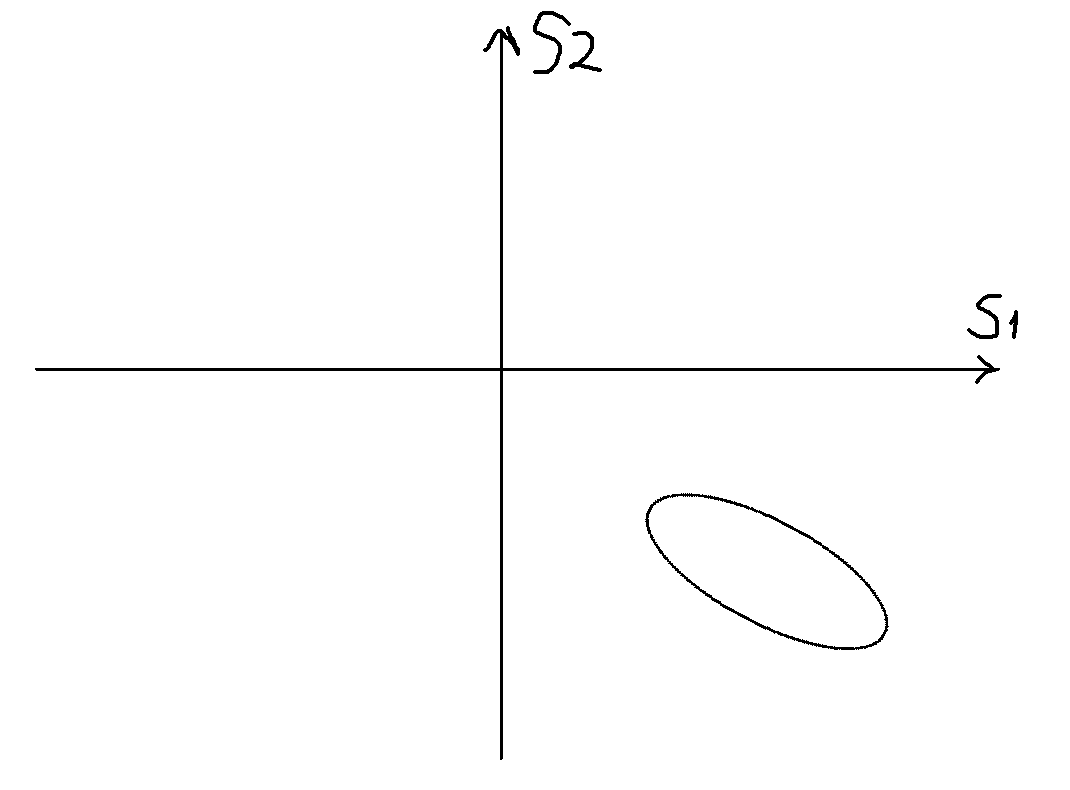
\includegraphics[width=0.5\linewidth]{./lect1/1.png}
\end{center}

\subsection{Lagrangian}
Let's describe the system with Lagrangian, which is function of coordinates, velocities and time.

Starting with one-particle system. Kinetic energy: $T(\dot{\vec{r}})=\frac{1}{2}m\dot{\vec{r}}^2$. Potential energy: $V(\vec{r}, t)$. Define
$$L(\vec{r}, \dot{\vec{r}}, t) = T(\dot{\vec{r}}) - V(\vec{r},t)$$
Derive Euler-Lagrange equations from Lagrangian:
$$\frac{d}{dt}\left( \frac{\partial}{\partial \dot{r}_\alpha} L(\vec{r}, \dot{\vec{r}}, t) \right) = \frac{\partial}{\partial r_\alpha} L(\vec{r}, \dot{\vec{r}}, t) $$
Since $L(\vec{r}, \dot{\vec{r}}, t) = T(\dot{\vec{r}}) - V(\vec{r},t)$:

$$\frac{\partial L}{\partial \dot{r}_\alpha} = \frac{\partial T}{\partial \dot{r}_\alpha} = \frac{\partial}{\partial \dot{r}_\alpha} \left[ \sum_{\beta} \frac{1}{2}m\dot{r}^2_p \right] = m\dot{r}\beta$$
$$\frac{d}{dt} \left( \frac{\partial L}{\partial \dot{r}_\alpha} \right) = m\ddot{r}_\alpha $$
$$\frac{\partial L}{\partial dr_\alpha} = -\vec{\nabla} V$$
We got Newton law:
$$m\ddot{\vec{r}} = -\vec{\nabla} V$$
\paragraph{Note} In different coordinates, $T$ might depend not only on velocities. For example, kinetic energy of a particle in spherical coordinates is $T = \frac{m}{2}\left[\dot{r}^2 + r^2\dot{\theta}^2 + r^2 \sin^2 \theta \cdot \dot{\varphi}^2 \right]$.

\paragraph{Multi particle system} For N particles:
$$L(\vec{r}_1,\dots, \vec{r}_N, \dot{\vec{r}}_1,\dots, \dot{\vec{r}}_N,t) = \sum_i \frac{1}{2} m_i \dot{\vec{r}}_i - V(\vec{r}_1,\dots, \vec{r}_N, t)$$

In this course we talk only on conserving forces. Meanwhile the potential is independent on velocity.

\paragraph{Example} Spring. $F_{spring} = kx$.
$$L(x, \dot{x}) = \frac{1}{2}m\dot{x}^2 - \frac{1}{2}kx^2$$
$$\frac{\partial L}{\partial x} = -kx$$

$$\frac{d}{dt}\left(\frac{\partial L}{\partial \dot{x}}\right) = \frac{d}{dt} m\dot{x} = m\ddot{x}$$

\subsection{Principle of least action}
Given the system described with Lagrangian
$$L(\vec{r}(t), \dot{\vec{r}}(t),t)= T_V$$
Lets take a look at path in configuration space:  \begin{wrapfigure}{R}{0.3\textwidth}
	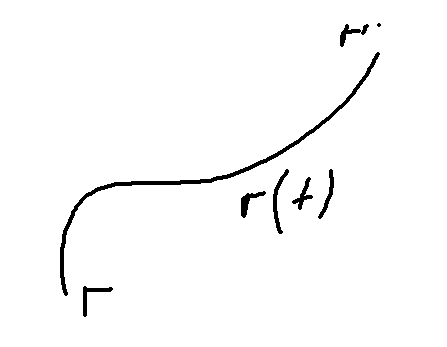
\includegraphics[width=\linewidth]{./lect1/2.png}
\end{wrapfigure}

Define action $S$ as
$$S\left[r(t)\right] = \int_{\tau_1}^{\tau_2} L(\vec{r}(t), \dot{\vec{r}}(t),t) dt$$
$S$ is functional, i.e. function whose parameter is function.
\paragraph{Note} Path $r(t)$ contains not only geometrical path but also the pace, i.e. if $q(\tau_1) = Q$ and $q(\tau_2)=Q^\prime$, there are different paths from $Q$ to $Q^\prime$ with different paces.
\paragraph{Principle of least action} Physical system described with Lagrangian $L$ will move in configuration space on path with minimal action $S$.

We'll show that Euler-Lagrange equations are necessary for existence of such path. We'll use principle of variation which is a way to find minimum of functional. Euler-Lagrange is acquired from principle of variation.
\subsection{Variational principle}
\subsubsection{How to find extremum of functional?}
First of all, how to find extremum of function? We need to find $x_0$ such that $\vec{\nabla} f = 0$.

For functional, lets choice different path between same points $q^\prime(t) = q(t) + \delta q(t)$. We can define a family of paths as $q(t) \to q(t)+u\cdot \delta q(t)$.

Define $g(u) = S\left[ q(t) + u \cdot \delta q(t) \right] = \int_0^\tau dt L(q(t) + u\cdot  \delta q(t), \dot{q}(t) + u\dot{\delta} q(t), t)$.

What is extremum of $g$?
$$\frac{dg}{du} = 0$$
$$\frac{dg}{du} = \frac{d}{du} \left( \int_0^\tau dt L(q(t) + u\delta q(t), q(t) + u\dot{\delta} q(t), t) \right) $$
Using Leibnitz rule, chain rule and denoting variable of Lagrangian as $q$. ($\frac{d}{du}\left[ q(t) + u\delta q(t)\right] = \delta q(t)  $ and also $\frac{d}{dq} \left[ q+\delta q \right] = 1$).
$$\frac{dg}{du} = \int_0^\tau dt \left[ \frac{\partial L}{\partial q} \delta q + \frac{\partial L}{\partial \dot{q}} \dot{\delta} q \right] $$
Integrating second term by parts ($f= \frac{\partial L}{\partial q}$ and $g = \frac{\partial q}{\partial u}$)
$$\frac{dg}{du} = \int_0^\tau dt \left[  \frac{\partial L}{\partial q} \delta q(t) - \delta q(t) \frac{d}{dt} \left(  \frac{\partial L}{\partial \dot{q}}  \right) \right] + \left[\frac{\partial L}{\partial \dot{q}} \delta q(t) \right]_0^\tau$$
Since $\delta q (0) = \delta q (\tau) = 0$:
$$\frac{dg}{du} = \int_0^\tau dt \left[ \frac{\partial L}{\partial q} - \frac{d}{dt} \left(  \frac{\partial L}{\partial \dot{q}}  \right) \right] \delta q(t) = 0$$
Since it is right for any $\delta q$,
$$\frac{\partial L}{\partial q} - \frac{d}{dt} \left(  \frac{\partial L}{\partial \dot{q}}\right) = 0$$
$$\frac{\partial L}{\partial q} = \frac{d}{dt} \left(  \frac{\partial L}{\partial \dot{q}}\right) $$
So Euler-Lagrange equation is equivalent to minimum of action.
\subsection{Principle of least action}
Given mechanical system with $N$ degrees of freedom described with Lagrangian:
$$L\left(q_1(t), \dots, q_n(t), \dot{q}_1(t), \dots, \dot{q}_n(t)\right)$$
The physical path of system in configuration space would be the path whose action 
$S\left[r(t)\right] = \int_{\tau_1}^{\tau_2} L(\vec{r}(t), \dot{\vec{r}}(t),t) dt$
would be minimal. The condition for that are Euler-Lagrange equations for each of degrees of freedom:
$$\frac{d}{dt}\left( \frac{\partial}{\partial \dot{q}_\alpha} L(\vec{r}, \dot{\vec{r}}, t) \right) = \frac{\partial}{\partial q_\alpha} L(\vec{r}, \dot{\vec{r}}, t) $$

\paragraph{Example}
Free particle:
$$L = T - V = \frac{m\dot{\vec{r}}}{2}$$
For 3D we have 3 equations:
$$\frac{d}{dt} \left( \frac{\partial L}{\partial \dot{r}_\alpha} \right) = \frac{\partial L}{\partial r_\alpha} $$
i.e.
$$\frac{d}{dt} \left( m\dot{r}_\alpha \right) = 0$$
$$m\ddot{\vec{r}} = 0$$
The solution is
$$\vec{r} = \vec{v}_0t+\vec{r}_0$$
Now lets calculate action on physical path. The Lagrangian of this path is $L = \frac{m\vec{v}_0^2}{2}$
$$ S\left[r(t)\right] = \int_{\tau_1}^{\tau_2} L(\vec{r}(t), \dot{\vec{r}}(t),t) dt = \frac{m\vec{v}_0^2}{2} \cdot \Delta t $$

Units of Lagrangian are $\left[\text{energy}\right]$ and of action $\left[\text{energy}\cdot \text{time} \right]$ 

Lets take different path:
$$\vec{r}(t) = \vec{r}_0 + \vec{v}_0 \Delta t \sin \left( \frac{\pi}{2\Delta t} t \right)$$
$$\dot{\vec{r}}(t) =\frac{\pi}{2} \vec{v}_0  \cos \left( \frac{\pi}{2\Delta t} t \right)$$
$$L(\vec{r}, \dot{\vec{r}}) = \frac{1}{2} \frac{\pi^2}{4}m \vec{v}_0^2  \cos^2 \left( \frac{\pi}{2\Delta t} t \right)$$
$$ S^\prime \left[r(t)\right] = \int_{\tau_1}^{\tau_2} L(\vec{r}(t), \dot{\vec{r}}(t),t) dt = \frac{\pi^2}{16} m\vec{v}_0^2  \cdot \Delta t  = \frac{\pi^2}{8}S\left[r(t)\right]$$

\paragraph{Different FOV}
Given FOV with velocity $\vec{v}_1$:
$$L^\prime = \frac{m}{2} \left( \dot{\vec{r}} - \vec{v}_1 \right)^2  = \frac{m}{2}\dot{\vec{r}} - m\dot{\vec{r}} + \frac{m}{2}\vec{v}_1^2$$
$$L^\prime  -L = - m\dot{\vec{r}} + \frac{m}{2}\vec{v}_1^2 $$

Define $F$ such that $\frac{dF}{dt} = L^\prime - L$:
$$F(\vec{r},t) =- m\vec{r} + \frac{m}{2}\vec{v}_1^2 t $$
Then
$$S^\prime \left[r(t)\right] = \int_{\tau_1}^{\tau_2} L(\vec{r}(t), \dot{\vec{r}}(t),t) + \frac{dF}{dt} dt =  S \left[r(t)\right] + \underbrace{\left( F(\tau_2) - F(\tau_1) \right)}_{\text{constant}}$$

Since addition of constant doesn't influence extremums, the solution doesn't changes.

Generally, we can define Lagrangian up to total derivative by time:
$$L^\prime  = L  + \frac{dF}{dt}$$
Basically that means we can drop everything that can be written as total derivative by time.
\subsection{Lagrangian formalism for conservative forces depending on velocity}
We can use Lagrangian formalism for conservative forces depending on velocity. Define generalized potential
$$U(\vec{r}, \dot{\vec{r}},t)$$
thus a Lagrangian is
$$L = T - U(\vec{r}, \dot{\vec{r}},t) $$
Then
$$\frac{d}{dt} \left( \frac{\partial L}{\partial \dot{r}_\alpha} \right) = \frac{\partial L}{\partial r_\alpha}$$
$$m\ddot{r}_\alpha - \frac{d}{dt} \left(  \frac{\partial U}{\partial \dot{r}_\alpha}  \right) = -  \frac{\partial U}{\partial r_\alpha} $$
Define
$$F_\alpha = \frac{d}{dt} \left(  \frac{\partial U}{\partial \dot{r}_\alpha}  \right)  -  \frac{\partial U}{\partial r_\alpha}$$

For example, for electromagnetic force we'll use potential
$$U = q \varphi(\vec{r},t) - q\vec{A} \left( \vec{r}, t \right) \dot{\vec{r}}$$

\section{Generalized coordinates}
Sometimes it's more convenient to use coordinate system different from Cartesian. For example if we have some kind of symmetry or restriction. Denote
$$q_a = q_a\left( r_\alpha^i, t \right)$$
And inverse is $r_\alpha^i(q_\alpha, t)$
Now we want to take derivative of $r$:
$$\frac{d}{dt} r_\alpha^i = \sum \frac{\partial  r_\alpha^i}{ q_a}\dot{q}_\alpha + \frac{\partial  r^i_\alpha}{ r}$$
We can rewrite Lagrangian as function of $q$, $\dot{q}$ and $t$ by substituting $\vec{r}$ and $\dot{\vec{r}}$: $ L(\vec{q}(t), \dot{\vec{q}}(t),t)$. In new coordinates
$$\frac{d}{dt}\left( \frac{\partial}{\partial \dot{q}_a} L(\vec{q}, \dot{\vec{q}}, t) \right) = \frac{\partial}{\partial q_a} L(\vec{q}, \dot{\vec{q}}, t) $$
\paragraph{Example}
Particle in 2D with potential $V(x,y)$:
$$L = \frac{1}{2}m(\dot{x}^2 + \dot{y}^2)-V(x,y)$$
$$\frac{d}{dt}\left( \frac{\partial L}{\partial \dot{x}} \right) = \frac{\partial L}{\partial x}$$
I.e.
$$m\ddot{x} = -\frac{\partial V}{\partial x}$$
$$m\ddot{y} = -\frac{\partial V}{\partial y}$$
In polar ($x=r\cos \theta$, $y=r\sin \theta$):
$$\dot{x} = \dot{r} \cos \theta - r\dot{\theta} \sin \theta$$
$$\dot{y} = \dot{r} \sin \theta + r\dot{\theta} \cos \theta$$
In Newtonian formalism we'd need $\ddot{x}$, which is often not trivial.

$$\dot{x}^2 + \dot{y}^2 = (\dot{r} \cos \theta - r\dot{\theta} \sin \theta)^2 + (\dot{r} \sin \theta + r\dot{\theta} \cos \theta)^2 = \dot{r}^2 + r^2 \dot{\theta}^2$$
Now
$$L(r,\dot{r},\theta,\dot{\theta}) = \frac{1}{2}(\dot{r}^2+r^2\dot{\theta}^2) - V(r, \theta)$$
Differentiating:
$$m\ddot{r} = mr\dot{\theta}^2 - \frac{\partial V}{\partial r}$$
$$2mr\dot{r}\dot{\theta} + mr^2 \ddot{\theta} = - \frac{\partial V}{\partial \theta}$$
\subsection{Constraints}
In some problem we have forces that constrain the movement of body. For example, movement on rope is 1D even though it happens in 3D. Rigid body keeps distance between its points constant. Molecules in the room are constrained to stay in the room. 
\paragraph{Holonomic constrains}
Constrain is called holonomic if it can be described with function
$$C(\vec{r}_1,\dots,\vec{r}_n, t) = 0$$

So if we have a bead on rope:
$$x^2+y^2=0$$
Or, for rigid body;
$$(x_2-x_1)^2 + (y_2-y_1)^2 = r_{12}^2$$
However, molecules in the room is non-holonomic constrain:
$$-L \leq x \leq L$$
\paragraph{bead on rotating rope}
Let's describe a particle sitting on a particular point on a bead.


\begin{center}
	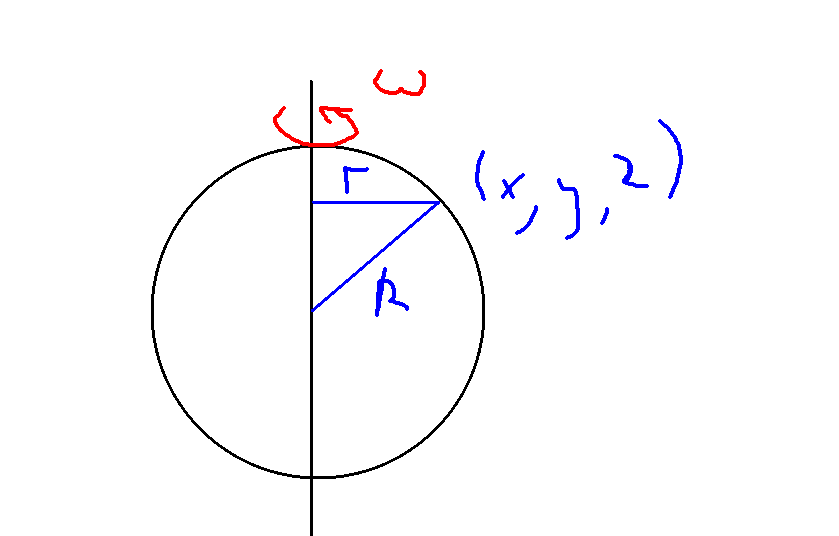
\includegraphics[width=0.5\linewidth]{./lect4/1.png}
\end{center}
We have two constraints. First is that particle on a sphere:
$$x^2+y^2+z^2-R^2 = 0$$
Second is that it doesn't move
$$(x,y,z) = (r\sin \omega t, r\cos \omega t, z) \Rightarrow x\cos \omega t - y\sin \omega t = 0$$

\subsubsection{Solving problems with constrains}
Given problem with $n$ degrees of freedom and $m$ constrains.

If $x_1, \dots, x_n$ are initial degrees of freedom.
and
$$\begin{cases} c_1(x_1, \dots, x_n, t) = 0 \\ \dots \\ c_m(x_1, \dots, x_n, t) = 0 \end{cases}$$

Effectively we have $n-m$ degrees of freedom. With movement equation
$$m\ddot{r} = \underbrace{F^i}_{Potential forces} + \underbrace{f^i}_{Constraining forces}$$
There are two way to solve constrained problem:
\begin{itemize}
	\item Find constrained plain, i.e. solve $3n-m$-dimensional problem. This is called D'Alembert's principle.
	\item Lagrange multipliers. Is useful when we cant find a parameterization for constrained plane or we want to see explicit constrains. This is $3n+m$-dimensional problem.
\end{itemize}

Constrained problem is
$$m\ddot{\vec{r}}_\alpha = F^i_\alpha + f^i_\alpha$$
where $i=1\dots n$ and $\alpha = 1,2,3$
The problems are that the coordinates aren't independent and that we don't know explicit constraining force.
\subsubsection{Solution with generalized coordinates}
$$L = T - V$$
is Lagrangian without constrains.
We add the constraining force:
$$\frac{d}{dt} \frac{\partial L}{\partial  \dot{r}^i_\alpha} - \frac{\partial L}{\partial  r^i_\alpha} =  f^i_\alpha $$

Note that $L$ isn't full Lagrangian since it doesn't includes constrains. We want every force to be conservative. The simple way guarantee that, we can choose all constraining forces to be orthogonal to the movement direction.

Define action
$$S\left[ \vec{r}(t) \right] = \int L dt$$
By perturbing the path:
$$\frac{d}{du} S\left[ \vec{r}(t) + u\delta \vec{r}(t)\right] = \int dt \left[\frac{d}{dt} \frac{\partial L}{\partial \partial \dot{r}^i_\alpha} - \frac{\partial L}{\partial  r^i_\alpha}\right] \delta  r^i_\alpha$$
But if $\vec{f} \perp \delta \vec{r}$, $\left[\frac{d}{dt} \frac{\partial L}{\partial \partial \dot{r}^i_\alpha} - \frac{\partial L}{\partial  r^i_\alpha}\right] \delta  r^i_\alpha = \vec{f} \cdot \delta \vec{r}= 0$, i.e. if we find a plane perpendicular to the constraining force, we can solve regular Euler-Lagrange equation.
\paragraph{Example}
Pendulum. 
$$L = \frac{1}{2} m(\dot{x}^2+\dot{y}^2) - mgy$$
By choosing $\theta$:
$$L(\theta, \dot{\theta}) = \frac{1}{2}ml^2 \dot{\theta}^2 -mgl(1-\cos \theta) = \frac{1}{2}ml^2 \dot{\theta}^2 + mgl\cos \theta$$
\paragraph{Example}
Pendulum connected to disk rotating with constant angular velocity $\omega$. Constrain is
$$c(x,y,t) = (r - R\sin \omega t)^2 + (r + R\cos \omega t)^2 - l^2$$
The Lagrangian is identical. 
$$L = \frac{1}{2} m(\dot{x}^2+\dot{y}^2) - mgy$$
The constrained plane is
$$x = R\cos \omega t + l\sin \theta $$
$$y = -R\sin \omega t - l\cos \theta $$
Differentiating:
$$\dot{x} = -R\sin \omega t +l\cos \theta \dot{\theta} $$
$$\dot{x} = -R\cos \omega t + l\sin \theta \dot{\theta} $$
Thus
$$L(\theta, \dot{\theta}, t) = \frac{1}{2}m\left( l^2\dot{\theta}^2 +R^2\omega^2 - 2R\omega l \dot{\theta}\sin \left(\omega t + \theta\right)\right) +mgR\sin \omega t +mgl \cos \theta$$
Since $mgR\sin \omega t = \frac{d}{dt} \left( \frac{mgR}{\omega} \cos \omega t \right)$
$$L(\theta, \dot{\theta}, t) = \frac{1}{2}m\left( l^2\dot{\theta}^2 +R^2\omega^2 - 2R\omega l \dot{\theta}\sin \left(\omega t + \theta\right)\right)  +mgl \cos \theta$$
$$ml\ddot{\theta}^2-mRl\omega\cos (\omega t +\theta)(\omega+\dot{\theta}) = -mR\omega l \dot{\theta} \cos (\omega t + \theta) - mgl\sin \theta$$
$$\ddot{\theta} = \frac{R\omega^2}{l} \cos (\omega t + \theta) - \frac{g}{l}\sin \theta$$

\subsubitem{Lagrange multipliers}
Lagrange multipliers is a way to solve optimization problem with constrains. 

Suppose we want to find minimum of function $f(x,y)$ under constrain $c(x,y)=0$.
Define function $g(x,y,\lambda) = f(x,y) - \lambda c(x,y)$
Lets find minimum of that function:
$$\begin{cases}
0 =&\frac{\partial g}{\partial x} = \frac{\partial f}{\partial x}  - \lambda \frac{\partial c}{\partial x} \\
0 =&\frac{\partial g}{\partial y} = \frac{\partial f}{\partial y}  - \lambda \frac{\partial c}{\partial y} \\
0 =&\frac{\partial g}{\partial \lambda} = c(x,y)
\end{cases}$$

Thus we can define new Lagrangian
$$L^\prime\left( r,\dot{r},\lambda_1(t), \dots, \lambda_m(t) \right) = L(r, \dot{r}, t) - \sum_{a=1}^m \lambda_a c_a(t)$$

Now define action:
$$S\left[ r(t), \lambda(t) \right] = \int dt L(r,\dot{r}, t) - \sum_{a=1}^m \lambda_a c_a(t)$$

The resulting Euler-Lagrange equations are
$$\begin{cases}
\frac{d}{dt} \frac{\partial L}{\partial \dot{r}_\alpha} = \frac{\partial L}{\partial r_\alpha} \underbrace{- \sum_a \lambda_a \cdot \frac{\partial c}{\partial r_\alpha}}_{\text{constraining force}}\\
0 =\frac{\partial L}{\partial \lambda_a}
\end{cases}$$

\paragraph{Example}
Pendulum in plane (no gravity).

$$L = \frac{1}{2} m\left( \dot{x} + \dot{y} \right)$$
Constrain
$$x^2+y^2-l^2 = 0$$
$$L^\prime (x,y,\dot{x}, \dot{y}, \lambda) = \frac{1}{2} m\left( \dot{x} + \dot{y} \right) - \lambda(x^2+y^2-l^2)$$

Deriving Euler-Lagrange:
$$\begin{cases}
m\ddot{x} = -2\lambda x\\
m\ddot{y} = -2\lambda y\\
x^2+y^2-l^2 = 0
\end{cases}$$

Solve the system:
$$mx\ddot{x} + my\ddot{y} = 2\lambda(x^2+y^2 ) = 2\lambda l^2$$
$$x\ddot{x} + y\ddot{y} = \frac{2\lambda l^2}{m}$$
After solving it we get
$$\lambda = \frac{1}{l^2} \frac{m(\dot{x}^2 + m\dot{y}^2)}{2} = \frac{E_k}{l^2}$$
Back to other equations
$$\begin{cases}
m\ddot{x} = -\frac{2E_k}{l^2} x\\
m\ddot{y} = -\frac{2E_k}{l^2} y\\
\end{cases}$$
Denote $\omega = \sqrt{\frac{2E_k}{ml^2}}$ acquiring
$$\begin{cases}
x = A \cos \left( \omega t + \varphi \right)\\
y = A \sin \left( \omega t + \varphi \right)
\end{cases}$$
\section{Conservation laws and symmetry}
Conserved value is
$$\frac{d}{dt} f(q,\dot{q}) = 0$$
\paragraph{Cyclic coordinate}
For $L(q,\dot{q},t)$ we define canonical momentum for each coordinate
$$p_i(q,\dot{q},t) = \frac{\partial L}{\partial \dot{q}_i}$$
Then Euler-Lagrange equations are
$$\frac{d}{dt} p_i = \frac{\partial L}{\partial q_i}$$

Cyclical coordinate are those for which canonical momentum  is conserved, i.e. Lagrangian doesn't depends on $q_i$.
\paragraph{Example}
Particle in plane with central force:
$$L = \frac{1}{2}m(\dot{x}^2 + \dot{y}^2)-V(x^2+y^2)$$
In polar:
$$L = \frac{1}{2}m(\dot{r}^2 + r^2 \dot{\theta}^2) - \vec{V}(r)$$
now
$$p_\theta = \frac{\partial L}{\partial \dot{\theta}} = mr^2\dot{\theta}$$
Then equations of movement are:
$$\begin{cases}
\frac{d}{dt} \left[ \frac{\partial L}{\partial \dot{r}} \right] = \frac{\partial L}{\partial r}\\
\frac{d}{dt} \left[ \frac{\partial L}{\partial \dot{\theta}} \right] = \frac{\partial L}{\partial \theta}\\
\end{cases}$$


$$\begin{cases}
m\ddot{r} = -\frac{\partial V}{\partial r} + mr\dot{\theta}^2\\
p_\theta = mr^2 \dot{\theta} := p_1
\end{cases}$$
i.e.
$$m\ddot{r} = -\frac{\partial V}{\partial r} + \frac{p_1^2}{mr^3}$$
We can solve this equation and obtain $r(t)$. From initial condition and $r(t)$, we can find $p_1$ and then find
$\theta(t) = \int \frac{p_1}{mr^2(t)}dt$
\paragraph{} If $q_n$ is cyclical coordinate $L(q_1, q_2,\dots,q_{n-1}, \dot{q}_1, \dot{q}_2,\dots, \dot{q}_n, t)$, then
$$p_n = \frac{\partial L}{\partial \dot{q}_n} = \text{const} = p$$
Then
$$\dot{q} = \dot{q} (q_1, q_2,\dots,q_{n-1}, \dot{q}_1, \dot{q}_2,\dots, t, p)$$
We can substitute it back to equations and solve them. After that we find $q_n(t)$ as
$$q_n(t) =\int \dot{q}_n (t) dt$$
\paragraph{Example}
Two particles with potential depending on distance between particles:
$$L = \frac{1}{2}m_1 \dot{\vec{r}}_1^2+\frac{1}{2}m_2 \dot{\vec{r}}_2^2 - V(\vec{r}_1 -\vec{r}_2)$$
By switching to $\vec{r} = \vec{r}_1 - \vec{r}_2$ and $\vec{R} = \vec{r}_1 + \vec{r}_2$ 
Then
$$L = \frac{1}{8}m_1 \left(\dot{\vec{R}} + \dot{\vec{r}}\right) +\frac{1}{8}m_1 \left(\dot{\vec{R}} - \dot{\vec{r}}\right)  - V(\vec{r})$$
Then
$$\vec{p}_R =\frac{1}{2}m_1\dot{\vec{r}}_1+\frac{1}{2}m_2\dot{\vec{r}}_2$$
\subsection{Connection between symmetry and conservation laws}
\paragraph{Noether's theorem}
Suppose we have continuous transformation with parameter $\alpha$: $q \to q_\alpha(q)$ such that $q = q_{\alpha = 0} (q)$. If Lagrangian is invariant under transformation, i.e.
$$L(\vec{q}_\alpha, \dot{\vec{q}}_\alpha,t)=L(\vec{q}, \dot{\vec{q}},t)$$
Then exists conserved value $\frac{dQ}{dt} = 0$.
$$Q = \sum \frac{\partial L}{\partial \dot{q}^i} \frac{\partial \dot{q}^i_\alpha}{\partial \alpha}_{\alpha = 0} = \sum_i p_i \frac{\partial \dot{q}^i_\alpha}{\partial \alpha}_{\alpha = 0}$$
\subparagraph{Proof}
\begin{align*}
0 = \frac{d L}{d \alpha}_{\alpha = 0} = \sum_i \left[ \frac{\partial L}{\partial q^i} \frac{\partial q^i}{\partial \alpha}_{\alpha = 0}+\frac{\partial L}{\partial \dot{q}^i} \frac{\partial \dot{q}^i}{\partial \alpha}_{\alpha = 0}\right] = 
\sum_i \left[ \frac{d}{dt}\left[\frac{\partial L}{\partial \dot{q}^i}\right] \frac{\partial q^i}{\partial \alpha}_{\alpha = 0}+\frac{\partial L}{\partial \dot{q}^i} \frac{d}{dt}\left[\frac{\partial q^i}{\partial \alpha}_{\alpha = 0}\right]\right] =\\= \sum_i \frac{d}{dt} \left[  \frac{\partial L}{\partial \dot{q}^i} \cdot \frac{\partial q^i}{\partial \alpha}_{\alpha = 0}\right] = \frac{d}{dt} \left[ \sum_i   \frac{\partial L}{\partial \dot{q}^i} \cdot \frac{\partial q^i}{\partial \alpha}_{\alpha = 0}\right] = \frac{dQ}{dt}
\end{align*}
\paragraph{Example}
$$q_\alpha(q) = \big( q_1+\alpha, q_2, \dots, q_n \big)$$
I.e. $q_1$ is cyclical, then $Q = p_1$.
\paragraph{Example}
Lagrangian which is independent on absolute positions (i.e. closed systems):
$$L = \frac{1}{2}m_i{\dot{ \vec{r}}^i}^2 - V(\vec{r}^i - \vec{r}^j)$$
Define $\vec{\lambda}$. The our transformation is
$$\vec{r}^i \to \vec{r}^i +\vec{\lambda}$$
Then
$$Q = \sum p_i \cdot \frac{\partial q_\lambda^i}{\partial \lambda}_{\lambda= 0} = \sum p_i = P_i$$
\paragraph{Example}
$$L = \frac{1}{2}m (x^2+y^2+z^2) - V(x^2+y^2+z^2)$$
Define rotation transformation
$$\begin{cases}
x_\alpha = x\cos \alpha + y\sin \alpha\\
y_\alpha = y\cos \alpha + x\sin \alpha\\
z= z
\end{cases}$$
$$\begin{cases}
\frac{\partial x_\alpha}{\partial \alpha}_{\alpha = 0} = y\\
\frac{\partial y_\alpha}{\partial \alpha}_{\alpha = 0} = -x\\
\frac{\partial z_\alpha}{\partial \alpha}_{\alpha = 0} = 0\\
\end{cases}$$

Then conserved value is
$$Q = \sum_i p_i \frac{\partial \dot{q}^i_\alpha}{\partial \alpha}_{\alpha = 0} = p_x \cdot y  - p_y \cdot x$$
Which is $z$ component of angular momentum.
\paragraph{Symmetry in time}
$$\frac{\partial L}{\partial t} = 0$$
Since
$$\frac{d L}{d t} = \sum_i \frac{\partial L}{\partial q^i} \dot{q} +  \frac{\partial L}{\partial \dot{q}^i} \ddot{q} = \sum_i \left[ \frac{d}{dt}  \left( \frac{\partial L}{\partial \dot{q}^i} \right) \dot{q}^i   \frac{\partial L}{\partial \dot{q}^i} \frac{d}{dt}\dot{q} \right] = \sum_i \left[ \frac{d}{dt} \left[ \frac{\partial L}{\partial \dot{q}_i}\dot{q}_i \right] \right] = \frac{d}{dt} \left[ \sum_i p_i \dot{q}_i \right]$$
Then
$$\frac{d}{dt} \left( \sum_i p_i \dot{q}^i - L \right) = 0$$
Denote
$$h = \sum_i p_i \dot{q}^i - L $$
It is called Jacobian integral.
If potential $V$ depends only on $q$, and
$$T(q, \dot{q}) = \frac{1}{2} \sum_{a,b} m_{ab}(q) \dot{q}^a \dot{q}^b$$
Then
$$p_i = \frac{\partial L}{\partial \dot{q}^i} = \frac{\partial T}{\partial \dot{q}^i} = \sum_i m_{ij} \dot{q}^i$$
$$\sum_i p_i \cdot \dot{q}^i  = \sum_{i,j} m_{ij} \dot{q}^i \dot{q}^j = 2T$$
$$h = \sum_i p_i \dot{q}^i - L = T + V$$
\section{Small Oscillations }
\subsection{1D harmonic oscillator}
Suppose $x_0$ is stable equilibrium. Write $V$ as a series around $x_0$:
$$V(x) = \underbrace{V(x_0)}_{0} + \underbrace{\frac{\partial V}{\partial x}_{x_0}\cdot (x-x_0)}_{0} + \frac{1}{2}\underbrace{\frac{\partial^2 V}{\partial x^2}_{x_0}}_{k}\cdot (x-x_0)^2$$
$$V(x) = \frac{1}{2}k(x-x_0)^2$$
Then, denoting $\eta = x - x_0$
$$L = \frac{1}{2}m\dot{\eta}^2 - \frac{1}{2} k \eta^2$$
From Euler-Lagrange:
$$m\ddot{\eta} = -k \eta$$
The solution is
$$\eta = C_1 \cos \omega t + C_2 \sin \omega t = A \cos (\omega t + \varphi)$$
In complex numbers
$$\eta = ae^{i \omega t} = A e^{i(\omega t + \varphi)}$$
Then 
$$a = A e^{i\varphi}$$
And
$$\ddot{\eta} = -\omega^2  A e^{i(\omega t + \varphi)}$$
\paragraph{Example}
Suppose following initial conditions: $\eta(0) = L$ and $\dot{\eta} = 0$
Then $A=L$ and $\varphi = 0$.
\subsection{$N$ non-coupled oscillators}
$$L  = \sum_i \left( \frac{1}{2}m_i\dot{\eta}_i^2  - \frac{1}{2} k_i  \eta_i^2\right)$$
Movement equations are:
$$\ddot{\eta}_i = -\frac{k_i}{m_i} \eta_i$$
$$\eta_i = a e^{i\omega_i t}$$
Define 
$$T = (T)_{ij}$$
In our case
$T_{ij} = \delta_{ij} m_i$
And define $$\eta = \begin{pmatrix}\eta_1 \\ \vdots \\ \eta_n\end{pmatrix}$$
And $V_{ij} = \delta_{ij} k_i$.

Then
$$T\dot{\eta} = \begin{pmatrix} \sum T_{1i}\eta_i \\ \vdots \\ \sum T_{Ni}\eta_i \end{pmatrix}$$ 
$$\dot{\eta}^T T\dot{\eta} = \sum_{i,j} T_{ij} \dot{\eta}_i \dot{\eta}_j$$
For our case $$\dot{\eta}^T T\dot{\eta} = \sum_{i,j} \delta_{ij} m_i \dot{\eta}_i \dot{\eta}_j = \sum_i m_i \dot{\eta}_i^2$$
and
$$\eta^T V \eta = \sum_i k_i \eta^2_i$$
$$L = \frac{1}{2} \dot{\eta}^T T\dot{\eta} + \frac{1}{2} \eta^T V \eta $$


\subsection{$N$ coupled oscillators}
Since potentials are now dependent of each other, lets write Taylor series:
$$V(\eta_1, \dots, \eta_N) = \underbrace{V_0}_{0} + \underbrace{\frac{\partial V}{\partial \eta_i}_{\eta=0} \eta_i}_{0} + \frac{1}{2}\frac{\partial^2 V}{\partial \eta_i \partial \eta_j}_{\eta=0} \eta_i \eta_j + \dots$$
Thus
$$V = \frac{1}{2} \frac{\partial^2 V}{\partial \eta_i \partial \eta_j}_{\eta=0} \eta_i \eta_j = \frac{1}{2} \eta^T V \eta$$
The potential matrix is
$$V_{ij} = \frac{\partial^2 V}{\partial \eta_i \partial \eta_j}$$

Now, for kinetic energy:
$$T = \sum_{i} \frac{1}{2} m_j \dot{\eta}^2_i$$
Then $T_{ij} = \delta_{ij} m_i$.

For generalized coordinates:
$$\dot{x}_i = \sum_j \frac{\partial x_i}{\partial q_j} \dot{q}_j$$
So
$$T = \frac{1}{2} \sum_i m_i \left( \sum_j \frac{\partial x_i}{\partial q_j} \dot{q}_j \right)^2 = \frac{1}{2} \sum_i m_i \sum_j \frac{\partial x_i}{\partial q_j} \dot{q}_j \sum_k \frac{\partial x_i}{\partial q_k} \dot{q}_k = \frac{1}{2} \sum_{j,k} \left( \underbrace{\sum_i m_i   \frac{\partial x_i}{\partial q_j} \frac{\partial x_i}{\partial q_k}}_{m_{jk}(q)}\right) \dot{q}_j \dot{q}_k $$

Since we all elements in $T$ are at least second-order , we can approximate $m_{jk}(q) = m_{jk}(0)$ since everything else is negligible:
$$T_{ij} = \frac{1}{2} \sum_{i,j} m_{jk_0} \dot{\eta}_j \dot{\eta}_k$$
i.e. $T_{jk} = m_{jk_0}$
We got the following Lagrangian:
$$L = \frac{1}{2} \dot{\eta}^T T \dot{\eta} - \frac{1}{2} \eta^T V \eta$$

From Lagrangian we derive $n$ motion equations:
$$\frac{d}{dt}\left[ \frac{\partial L}{\partial \dot{\eta}_k} \right] = \frac{\partial T}{\partial \eta_k}$$ 
$$\frac{\partial L}{\partial \dot{\eta}_k} = \frac{\partial T}{\partial \dot{\eta}_k} = \frac{1}{2}  T_{kj} \dot{\eta}_j \frac{1}{2}  T_{ki} \dot{\eta}_i =  T_{ki} \dot{\eta}_i   $$
$$\frac{d}{dt}\left[ \frac{\partial L}{\partial \dot{\eta}_k} \right]  = T_{ki} \ddot{\eta}_i$$
$$\frac{\partial T}{\partial \eta_k} = -\frac{\partial V}{\partial \eta_k} = -V_{ki} \eta_i$$

Thus
$$ T_{ki} \dot{\eta}_i = -V_{ki} \eta_i$$  
In matrix form
$$T \ddot{\eta} = -V \eta$$

\paragraph{Simple case}
In simple case $T_{ji} = m_j \delta_{ji}$ and $V_{ji} = k_i \delta_{ji}$. The equation is 
$$m_i\ddot{\eta}_i = -k_i \eta_i$$
$$\eta_i = a+i e^{-i\omega t}$$

\subsubsection{Diagonalization of the problem}
We'll show that there is coordinates such that both $T$ and $V$ are diagonal, and thus the problem is simple in this set of coordinates.
\paragraph{Finding eigenfrequencies}
$$T_{kj} \ddot{\eta}_k + V_{kj} \eta_j = 0$$
Guess solution
$$\eta_k = ca_k e^{-i\omega t}$$
$$\ddot{\eta}_k = -\omega^2 ca_k e^{-i\omega t}$$
Thus
$$\omega^2 T_{kj} a_j = V_{kj} a_j$$
$$(V-\omega^2T)a = 0$$

We have solution $a \neq 0$ if $ \det V-\omega^2 T = 0$.
Denote $\lambda_1,\dots,\lambda_n$ solutions of this equation, i.e. $\omega_k^2 = \lambda_k$ such that $ \det V-\omega^2 T = 0$. and vector $\vec{a}_k \neq 0$ such that 
$(V-\omega^2T)a = 0$.


Lets show that $\lambda_k$ is real and positive, thus $\omega_k$ describes oscillations of the system. 
$$(V-\omega^2T)a = 0$$
$$a^\dagger(V-\omega^2T)a = 0$$
where $*$ is complex conjugate and $\dagger$ is transposed complex conjugate. 
$$\omega^2 = \frac{a^\dagger V a}{a^\dagger T a}$$

Lets look on 
$$\left(a^\dagger V a\right)^* = a^T {V^T}^* a^*$$
But $V^\dagger = V$, since it real and symmetric:
$$\left(a^\dagger V a\right)^*  = a^\dagger V a$$
i.e. $a^\dagger V a$ is real.

Denote $a = \alpha + i \beta$.
$$a^\dagger V a = \left(\alpha - i \beta\right)^TV\left(\alpha + i \beta\right) = \alpha^T V \alpha + \beta^T V \beta $$
Since we are looking at steady equilibrium, $V$ is positive around it, and thus the whole thing is positive. 

We can do the same for $T$, and $T$ is positive since it's kinetic energy. 

If $V<0$ (for example, unstable equilibrium), the solution isn't oscillator. We get complex number substituted in exponent, acquiring real exponent.

We acquired $N$ eigenfrequencies and $N$ corresponding eigenvectors.

Then general solution is
$$\eta(t) = \sum_j c_j a_j e^{i\omega_j t}$$
In matrix form, if we denote $A(t) = \left(a_{j\downarrow} e^{i\omega_j t}\right)_{kj}$ i.e. matrix of columns of mode solutions:
$$\eta(t) = A(t)\vec{c} $$

\paragraph{Example}
A system of three springs and two masses. Denote $x_1$ and $x_2$ the displacement of masses from equilibrium. Denote middle spring as $k_3$.
$$T = \frac{1}{2}m_1\ddot{x}_1+\frac{1}{2}m_2\ddot{x}_2$$
$$V = \frac{1}{2}k_1x_1^2+\frac{1}{2}k_2x_2^2+\frac{1}{2}k_3(x_1-x_2)^2 = \frac{1}{2} (k_1+k_3)x_1^2 +  \frac{1}{2} (k_2+k_3)x_2^2 - k_3 x_1x_2$$
Then in matrix form:
$$T  = \begin{pmatrix}
m_1&0\\0&m_2
\end{pmatrix}$$
$$V  = \begin{pmatrix}
k_1+k_3&-k_3\\-k_3&k_2+k_3
\end{pmatrix}$$

To find eigenfrequencies we need
$$(V - \omega^2 T) \vec{a} = 0$$
$$V - \omega^2 T =  \begin{pmatrix}
k_1+k_3-\omega^2m_1&-k_3\\-k_3&k_2+k_3-\omega^2m_2
\end{pmatrix}$$

$$\det (V - \omega^2 T) = (k_1+k_3-\omega^2m_1)(k_2+k_3-\omega^2m_2) - k_3^2 = 0$$
If $K_1=k_2=k_3$ and $m_1=m_2$:
$$(2k-\omega^2m)^2 = k^2$$
$$2k - \omega^2 m = \pm k$$

$$ \begin{cases}
\omega^2_1 =\frac{3k}{m}\\
\omega^2_2 =\frac{k}{m}\\
\end{cases}$$

Now lets find eigenvectors:
$$\begin{pmatrix}
-k & -k\\-k&-k
\end{pmatrix} \alpha_1 = 0$$


$$\begin{pmatrix}
k & -k\\-k&k
\end{pmatrix} \alpha_2 = 0$$


\subsection{Switch to normal coordinates}
Normal coordinates are coordinates in which $T$ and $V$ are diagonal.
Since
$$V\vec{a}_k = \lambda_k T \vec{a}_k$$
$$\vec{a}_l^TV = \lambda_l \vec{a}_l^T T $$
$$(\lambda_k - \lambda_l) \vec{a}_l^T T \vec{a}_k = \vec{a}_l^TV\vec{a}_k -\vec{a}_l^TV\vec{a}_k = 0 $$

Suppose that all eigenvalues are different, then
$$\vec{a}_l^T T \vec{a}_k = 0$$
If we take matrix $A  =\begin{pmatrix} \vec{a}_1, \vec{a}_2, \dots, \vec{a}_n \end{pmatrix}$
then 
$$A^TTA=I$$
Now lets show that
$$A^TVA=\lambda$$
where $\lambda$ is matrix with eigenvalues on diagonal.

Now, since $V\vec{a}_k = T \vec{a}_k\lambda_k $,
$$VA  =TA\lambda$$
$$A^TVA  =A^TTA\lambda  =I\lambda = \lambda$$

Define normal coordinates
$$\vec{\eta} = A\vec{\xi}$$

Then
$$V = \frac{1}{2} \eta^T V \eta = \frac{1}{2} \xi^T A^T V A \xi = \frac{1}{2} \xi^T \lambda \xi$$
$$T = \frac{1}{2} \eta^T T \eta = \frac{1}{2} \xi^T A^T T A \xi = \frac{1}{2} \xi^T \xi$$

Now we have non-coupled equations:
$$L = \frac{1}{2} \sum_K \left(  \dot{\xi}_k^2 - \omega^2_k \xi^2_k \right)$$
, thus
$$\ddot{\xi}_k+ \omega_k^2 \xi_k = 0$$
with solution
$$\xi_k = c_k e^{-i\omega_k t}$$
$$\xi = \begin{pmatrix}c_1 e^{-i\omega_1 t}\\c_2 e^{-i\omega_2 t}\\\vdots \\ c_n e^{-i\omega_n t}\\\end{pmatrix}$$

\paragraph{Back to example of coupled oscillator}
Normalizing eigenvalues by $\frac{1}{\sqrt{2m}}$
$$A = \frac{1}{\sqrt{2m}} \begin{pmatrix} 1&1\\-1&1\end{pmatrix}$$
and
$$\begin{pmatrix}
x_1\\x_2
\end{pmatrix} = A \begin{pmatrix} \xi_1\\\xi_2 \end{pmatrix}$$
Then
$$A^T T A = \frac{1}{\sqrt{2m}} \begin{pmatrix} 1&-1\\1&1\end{pmatrix} \begin{pmatrix}m&0\\0&m\end{pmatrix} \frac{1}{\sqrt{2m}}\begin{pmatrix} 1&1\\-1&1\end{pmatrix} = \frac{1}{2m} \begin{pmatrix}2m&0\\0&2m\end{pmatrix}  = I$$
$$A^TVA =  \begin{pmatrix}\frac{3k}{m}&0\\0&\frac{k}{m}\end{pmatrix} =  \begin{pmatrix}\omega_1^2&0\\0&\omega_2^2\end{pmatrix}$$
The Lagrangian is
$$L = \frac{1}{2} \left( \dot{\xi}^2_k - \omega^2_k \xi^2_k \right)$$
$$\xi(t) = \begin{pmatrix} c_1e^{-i\omega_1 t} \\c_2e^{-i\omega_2 t} \end{pmatrix}$$
For initial conditons $\vec{x}(t) = \begin{pmatrix}\delta x \\ 0\end{pmatrix}$ and $\dot{\vec{x}}(t) = \begin{pmatrix}0 \\ 0\end{pmatrix}$.

In normal coordinates
$\dot{\vec{\xi}} = \begin{pmatrix}\frac{\lambda x}{2} \sqrt{2m} \\\frac{\lambda x}{2} \sqrt{2m}\end{pmatrix}$ and  $\dot{\vec{\xi}}(t) = \begin{pmatrix}0 \\ 0\end{pmatrix}$.

Then $c_1=c_2$ and $c_1+c_2 = \delta x$.
$$c_1=c_2 = \frac{\delta x}{2}$$
\section{Hamiltonian formalism}
In Hamiltonian formalism we want to describe system with positions and momenta. Momentum connected with coordinate $q_i$ is
$$p_i(q,\dot{q},t) = \frac{\partial L}{\partial \dot{q}}$$
We want to find inverse transformation $\dot{q}(q,p,t)$. It's possible iff $$0 = \left| \frac{\partial p_1}{\partial \dot{q}_j} \right| = \left| \frac{\partial^2 L}{\partial \dot{q}_i \dot{q}_j} \right|$$

Define Hamiltonian
$$H(\vec{q}, \vec{p}, t) = \sum_i p_i\dot{q}_i(\vec{q}, \vec{p}, t) - L \big(q, \dot{q}_i(\vec{q}, \vec{p}, t) , t \big)$$

\paragraph{Examples}
\subparagraph{Free particle}
$$L = \frac{m \dot{q}^2}{2}$$
$$p = m\dot{q} \Rightarrow  \dot{q} =  \frac{p}{m}$$
$$H = \frac{p^2}{2m}$$
\subparagraph{Harmonic oscillator}
$$L = \frac{m\dot{q}^2}{2} - \frac{kq^2}{2}$$
$$H = \frac{p^2}{2m} + \frac{kq^2}{2}$$
\subparagraph{General potential in 3D in Cartesian}
$$L = \frac{1}{2} m\left(\dot{x}^2+\dot{y}^2+\dot{z}^2\right)- V(x,y,z)$$
$$H = \frac{p_x^2+p_y^2+p_z^2}{2m} + V(x,y,z)$$
\subparagraph{General potential in 3D in spherical}
$$L = \frac{1}{2} m\left(\dot{r}^2+r^2\dot{\theta}^2+r^2\sin^2 \theta \dot{\varphi}^2\right)- V(r,\theta, \varphi)$$
$$\begin{cases}
p_r = m\dot{r}^2\\
p_\theta = mr^2 \dot{\theta}\\
p_\varphi = mr^2\sin^2\theta \dot{\varphi}
\end{cases}$$
\begin{align*}
H = p_r\dot{r} + p_\theta \dot{\theta} +p_\varphi \dot{\varphi} - L = \frac{p_r^2}{m}+\frac{p_\theta^2}{mr^2}+\frac{p_\varphi^2}{mr^2\sin^2\theta} -\frac{1}{2} m\left(\frac{p_r^2}{m^2}+\frac{p_\theta^2}{m^2r^2}+\frac{p_\varphi^2}{m^2r^2\sin^2\theta}\right)+ V(r,\theta, \varphi)  =\\= \frac{1}{2m} \left(p_r^2+\frac{p_\theta^2}{r^2}+\frac{p_\varphi^2}{r^2\sin^2\theta}\right)+ V(r,\theta, \varphi)
\end{align*}


\paragraph{N particles without interaction}
$$L = \sum_i \frac{1}{2}m_i \dot{\vec{r}}_i^2 - V(\vec{r}_i) = \sum_{\alpha, i} \frac{1}{2}m_i {\dot{\vec{r}}_i^\alpha}^2 - V(\vec{r}_i)$$
$$H = \sum_{\alpha, i}  \frac{{p_i^\alpha}^2}{2m_i} + \sum V(r_i)$$
\subsection{Movement equations in Hamiltonian formalism}
$$dH = \sum_i \frac{\partial H}{\partial q_i}dq_i+\sum_i \frac{\partial H}{\partial p_i}dp_i+ \frac{\partial H}{\partial t}dt$$

On the other hand
\begin{align*}
dL =  \sum_i \frac{\partial L}{\partial q_i}dq_i+\sum_i \frac{\partial L}{\partial\dot{q}_i}d\dot{q}_i+ \frac{\partial L}{\partial t}dt = \sum_i \frac{d}{dt}\frac{\partial L}{\partial \dot{q}_i}dq_i+\sum_i \frac{\partial L}{\partial\dot{q}_i}d\dot{q}_i+ \frac{\partial L}{\partial t}dt =\\= \sum_i \dot{p}_i dq_i+\sum_i p_i d\dot{q}_i+ \frac{\partial L}{\partial t}dt = \sum_i \dot{p}_i dq_i+\underbrace{d \left(\sum_i p_i \dot{q}_i\right)}_{=\sum_i \dot{q}_i d p_i+\sum_i \dot{p}_i d q_i}- \sum_i \dot{q}_i d p_i+ \frac{\partial L}{\partial t}dt
\end{align*}
$$dH = d\left( \sum p_i \dot{q}_i - L \right) = -\sum \dot{p_i} dq_i + \sum \dot{q}_i dp_i - \frac{\partial L}{\partial t}dt$$

Thus
$$\begin{cases}
\dot{p}_i = -\frac{\partial H}{\partial q_i} \\
\dot{q} = \frac{\partial H}{\partial p_i}
\end{cases}$$

\paragraph{Equivalence of Hamilton and Euler-Lagrange equations}
$$\dot{p}_i = \frac{d}{dt} \frac{\partial L}{\partial \dot{q}_i}_{q=\text{const}}=  \frac{\partial L}{\partial q_i}_{\dot{q}=\text{const}}$$
$$\frac{\partial L}{\partial q_i}_{p=\text{const}}=\frac{\partial L\big( q, \dot{q}(q,p,t),t \big)}{\partial q_i}_{p=\text{const}}=\frac{\partial L}{\partial q_i}_{\dot{q}=\text{const}} + \sum_j \frac{\partial L}{\partial \dot{q}_j}\frac{\partial \dot{q}_j}{\partial q_i}_{p=\text{const}}$$
Thus
$$\dot{p}_i = \frac{\partial L}{\partial q_i}_{p=\text{const}} - \sum_j p_j\frac{\partial \dot{q}_j}{\partial q_i}_{p=\text{const}} = -\frac{\partial }{\partial q_i}\left[ \sum p_j \dot{q}_j - L \right]_{p=\text{const}} = -\frac{\partial H}{\partial q_i}_{p=\text{const}}$$


\paragraph{Examples of Hamilton equations}
\subparagraph{Free particle}
$$H = \frac{p^2}{2m}$$
$$\dot{p} = 0 \Rightarrow p = p_1$$
$$\dot{q}=  \frac{p_0}{m}$$
$$q(t) = \frac{p_0}{m}t+q_0$$
\subparagraph{harmonic oscillator}
$$H = \frac{p^2}{2m} + \frac{kq^2}{2}$$
$$p = -\frac{\partial H}{\partial q} = -kq$$
$$\dot{q} = \frac{\partial H}{\partial p} = \frac{p}{m}$$
$$\ddot{q} = -\frac{k}{m}q$$
\subparagraph{N particles without interaction}
$$H = \sum_{i, \alpha} \frac{{p_i^\alpha}^2}{2m_i} + \sum_i V(\vec{r}_i)$$
$$\dot{r}_i^\alpha = \frac{p_i^\alpha}{m_i}$$
$${\dot{p}_i^\alpha} = -\frac{\partial V(\vec{r}_i)}{\partial r^\alpha_i}$$
Thus
$$m\ddot{r}_i^\alpha=-\frac{\partial V(\vec{r}_i)}{\partial r^\alpha_i}$$
\subsection{Phase space}
Given $n$ degrees of freedom, phase space is $2n$-dimensional space, where coordinates are position and momentum. Each point uniquely describes state of the system. Pathes in phases space can't intersect.
\paragraph{Liouville's theorem }
In phase space volume is conserved in time. 

\subsection{Switching between Lagrangian and Hamiltonian}

The switch is a case of Legendre transform.
\paragraph{Legendre transformation}
Suppose we have $f(x)$ and $y=f^\prime(x)$, define $g(y)$ - Legendre transformation of $f(x)$:
$$g(y) = y \cdot x(y) - f(x(y))$$
$$\frac{dg}{dy} = x(y) + yx^\prime(y) - \frac{df}{dx} \frac{dx}{dy} = x(y) + yx^\prime(y) -yx^\prime(y) = x(y)$$
Thus $x = g^\prime(x)$ and we can perform Legendre transformation of $g(y)$:
$$\tilde{f}(x)= y(x) x - g(y(x)) = yx - (yx - f(x)) = f(x)$$
\paragraph{Example}
$$f(x) = ax^2 \Rightarrow y = 2ax \Rightarrow x= \frac{y}{2a}$$
$$g(y) = yx- f(x) = \frac{y}{2a}y  -a \left(\frac{y}{2a}\right)^2 = \frac{y^2}{4a}$$
\paragraph{Example}
$$f(x) = e^x \Rightarrow y = e^x \Rightarrow x= \ln y$$
$$g(y) = yx- f(x) = y\ln y  - y = y (\ln y -1)$$
\subsection{Lagrangian}
In this case $x$ is $\dot{q}$ and $y$ is $p$.
If we perform Legendre transformation on $L$ we get $H$:
$$H = \sum p_i \dot{q}_i - L$$

\subsection{Poisson bracket}
Given $f(q,p,t)$, and its total derivative by time:
$$\frac{df}{dt} = \sum_i \left( \frac{\partial f}{\partial q_i} \frac{dq_i}{dt} + \frac{\partial f}{\partial p_i} \frac{dp_i}{dt}  \right) + \frac{\partial f}{\partial t} = \sum_i \left( \frac{\partial f}{\partial q_i} \frac{\partial H}{\partial p_i} + \frac{\partial f}{\partial p_i} \frac{\partial H}{\partial q_i}  \right) + \frac{\partial f}{\partial t}$$

\paragraph{Poisson bracket}
Given $f(q,p,t)$ and $g(q,p,t)$ define  Poisson bracket
$$\left\{ f,g \right\} = \sum_i \left( \frac{\partial f}{\partial q_i} \frac{\partial g}{dp_i} + \frac{\partial f}{\partial p_i} \frac{\partial g}{\partial q_i}  \right)$$
Then we get
$$\frac{df}{dt} = \left\{ f, H \right\} + \frac{\partial f}{\partial t}$$

If $f$ isn't explicitly dependent on time, then
$$\left\{ f,H \right\} =0 \iff f \text{ conserved}$$

\paragraph{Properties of Poisson brackets}
\begin{itemize}
	\item Anticommutativity: $$\{f, g\} = -\{g, f\}$$
	\item  Bilinearity: $$\{af + bg, h\} = a\{f, h\} + b\{g, h\}, \quad \{h, af + bg\} = a\{h, f\} + b\{h, g\}, \quad a, b \in \mathbb R$$
	\item  Product rule(Leibniz's rule): $$\{fg, h\} = \{f, h\}g + f\{g, h\}$$
	\item  Jacobi identity: $$\{f, \{g, h\}\} + \{g, \{h, f\}\} +  \{h, \{f, g\}\} = 0$$
\end{itemize}

Also, if a function $k$ is constant over phase space (but may depend on time), then $\{f,\, k\} = 0$ for any $f$.

\paragraph{Note}
Movement equations are particular case of 
$$\frac{df}{dt} = \left\{ f,H \right\} + \frac{\partial f}{\partial t} $$

Taking $f=q$:
$$\dot{q} = \left\{ q_i, H \right\} = \sum_i \left( \frac{\partial q_i}{\partial q_i} \frac{\partial H}{\partial p_i} + \frac{\partial q_i}{\partial p_i} \frac{\partial H}{\partial q_i}  \right) = \frac{\partial H}{\partial p_i}$$
$$\dot{q} = -\frac{\partial H}{\partial q_i}$$

\paragraph{Note}
\begin{align*}
\{q_i,q_j\} &= 0 \\
\{p_i,p_j\} &= 0 \\
\{q_i,p_j\} &= \delta_{ij}
\end{align*}

\paragraph{Claim}
If $f$ and $g$ are conserved, then $h=\left\{ f,g \right\}$ is conserved too.
\subparagraph{Proof}
$$\left\{ h,H \right\} = \big\{ \left\{f,g \right\}, H \big\} = - \big\{ \left\{g,H \right\}, f \big\} - - \big\{ \left\{H,f \right\}, g \big\}  = 0$$

\paragraph{Example}
$$H = \frac{\vec{p}^2}{2m} + V(\vec{r})$$
We know that angular momentum in directions $x$ and $y$ are conserved:
$$l_x = yp_z-zp_y$$
$$l_y = zp_x - xp_z$$
We know that $\{ l_x, l_y \}$ is conserved too.

$$\left\{ l_x, l_y \right\} = \left\{ yp_z - zp_y, zp_x - xp_z \right\}$$

Opening by bilinearity and then as product:
$$\left\{ yp_z, zp_x  \right\} =\left\{ yp_z, z  \right\}p_x + \left\{ yp_z, p_x \right\}z = \underbrace{\left\{ y, z  \right\}}_{0}p_zp_x + \left\{ p_z, z  \right\}yp_x + \underbrace{\left\{ y, p_x \right\}}_{0}p_zz+ \underbrace{\left\{p_z, p_x \right\}}_{0} yz  $$
Thus

$$\left\{ l_x, l_y \right\} = \left\{ yp_z - zp_y, zp_x - xp_z \right\} = yp_x\left\{ p_z, z \right\} + xp_y \left\{ z,p_z \right\} = -yp_x + xp_y = l_z$$
\subsection{Cyclical coordinates in Hamiltonian formalism}
\paragraph{Example}
$$L = \frac{1}{2}m \left( \dot{r}^2 + r^2\dot{\theta}^2 \right) + V(r)$$
$\theta$ is cyclical coordinate since Lagrangian doesn't depends on $\theta$. Also
$$p_\theta = mr^2\dot{\theta}$$
$$p_r = m\dot{r}$$
i.e.
$$H = p_r\dot{r} + p_\theta \dot{\theta} - L  = \frac{p_r^2}{2m} + \frac{p_\theta^2}{2mr^2} + V(r)$$

\paragraph{Definition}
Coordinate is cyclical  if $\frac{\partial H}{\partial \dot{q}} = 0$. Coordinate is cyclical in Hamiltonian formalism iff it is cyclical if Lagrange formalism.
\begin{align*}
\frac{\partial H}{\partial q_i}_{p,t=\textmd{const}} = \frac{\partial}{\partial q_i} \left[  p_j\dot{q}_j - L(q,\dot{q},t)\right]_{p=\textmd{const}} = p_j \frac{\partial \dot{q}_j}{\partial q_i}_{p=\textmd{const}} - \frac{\partial L}{\partial q_i}_{\dot{q}=\textmd{const}} - \frac{\partial L}{\partial \dot{q}_j}\frac{\partial \dot{q}_j}{\partial q_i}_{p=\textmd{const}} =\\= p_j \frac{\partial \dot{q}_j}{\partial q_i}_{p=\textmd{const}} - \frac{\partial L}{\partial q}_{\dot{q}=\textmd{const}} - p_j\frac{\partial \dot{q}_j}{\partial q_i}_{p=\textmd{const}} = - \frac{\partial L}{\partial q}_{\dot{q}=\textmd{const}} 
\end{align*}

\paragraph{Example}
Suppose $i$ is cyclical coordinates. We can reduce one degree of freedom: $$H(q_1, q_2, \dots, q_\alpha, \dots, q_n, p_1, \dots, p_\alpha, \dots, p_n, t) = H_\alpha(q_1, q_2, \dots, q_n, p_1, \dots, p_n, t)$$. Solving this problem we get $q_i$ and $p_i$ as a function of alpha, and
$$\dot{q}_i = \frac{\partial H}{\partial p_i} = \frac{\partial H_\alpha}{\partial p_\alpha}$$
$$q_i= q_{i0} + \int_0^t  \frac{\partial H_\alpha}{\partial p_\alpha} dt^\prime $$
\paragraph{Notation}
$$(q_1, q_2, \dots, q_n, p_1, \dots, p_n)= \left(n_1, \eta_2, \dots, \eta_{2n} \right)$$
Define block matrix $J$:
$$J = \begin{pmatrix}
0&I_{n\times n}\\-I_{n\times n} & 0
\end{pmatrix}$$
$J$ is antisymmetric (where gradient is row vector).
$$\dot{\vec{\eta}} = J \nabla_{\vec{\eta}} H^T$$

Then
$$\left\{ f(\eta), g(\eta) \right\} = \nabla_{\vec{\eta}}  f J \nabla_{\vec{\eta}}  g^T$$

\subsection{Canonical transformation}
$(q,p) \to (q^\prime, p^\prime)$ $\Rightarrow$ $\eta \to \eta^\prime$.
In contrast to Lagrangian formalism, we can mix momenta and coordinates in our transformations. However, we want to limit ourselves to coordinates for which movement equations are fulfilled:
$$\dot{q}^\prime_i = \frac{\partial H^\prime}{\partial p^\prime_i} \quad \dot{p}^\prime_i = -\frac{\partial H^\prime}{\partial q^\prime_i}$$
Such transformation is called canonical transformation.
\paragraph{1D oscillator}
$$L = \frac{1}{2}m\dot{q}^2 - \frac{1}{2}kq^2$$
Define $\omega^2 = \frac{k}{m}$:
$$H = \frac{p^2}{2m} + \frac{kq^2}{2}$$
Define transformation 
$$\begin{cases}
q = \sqrt{\frac{2p}{m\omega}} \sin q^\prime\\
p = \sqrt{2m\omega p} \cos q^\prime\\
\end{cases}$$
i.e.
$$\begin{cases}
q^\prime = \arccot \frac{p}{2ma}\\
p^\prime = \frac{p^2}{2m\omega} + \frac{q^@m\omega}{2} = \frac{1}{2m\omega} \left(p^2+m\omega^2 q^2\right) \\
\end{cases}$$

Then
$$H =\omega p^\prime$$
Then $\dot{q}^\prime = \omega$ and $\dot{p}^\prime = 0$, meaning
$$\begin{cases}
q^\prime(t) = q_1^\prime + \omega t\\
p^\prime(t) = \frac{E}{\omega}
\end{cases}$$
Those coordinates are basically phase and amplitude.

\paragraph{When transformation is canonical}
%TODO vectors
Suppose we have transformation $\eta \to \eta^\prime$ such that
$$\dot{\vec{\eta}}^\prime = J \nabla_{\vec{\eta}^\prime} H^T$$
Since
$$H^\prime(\eta^\prime) = H\big( \eta (\eta^\prime) \big) $$
$$\frac{\partial H^\prime}{\partial \eta^\prime_k} = \sum_m \frac{\partial H}{\partial \eta_m}\frac{\partial \eta_m}{\partial \eta_k}$$
That means
$$\dot{n}_i^\prime =  \sum_j \frac{\partial \eta^\prime_i}{\partial \eta_j} \dot{\eta}_j= \sum_{j,k} \frac{\partial \eta^\prime_i}{\partial \eta_j} J_{jk} \frac{\partial H}{\partial \eta_k} = \sum_m \left(\sum_{j,k}\frac{\partial \eta^\prime_i}{\partial \eta_j}  J_{jk}  \frac{\partial \eta^\prime_m}{\partial \eta_k}\right)\frac{\partial H^\prime}{\partial \eta^\prime_m}$$

And we want
$$\dot{\eta}_i^\prime = \sum_m J_{im} \frac{\partial H^\prime}{\partial q^\prime_m}$$ 
i.e.
$$J_{im} = \sum_{j,k}\frac{\partial \eta^\prime_i}{\partial \eta_j}  J_{jk}  \frac{\partial H}{\partial \eta_k} \Rightarrow D_{\vec{\eta}} \vec{\eta^\prime} \cdot J \cdot D_{\vec{\eta}} \vec{\eta^\prime}^T  = J$$ 
where $D_{\vec{\eta}} \vec{\eta^\prime}$ is differential of $\vec{\eta^\prime}$ by $\vec{\eta}$:
$$D_{\vec{\eta}} \vec{\eta^\prime} = \begin{pmatrix}
\frac{\partial \eta^\prime_1}{\partial \eta_1}  & \dots & \frac{\partial \eta^\prime_1}{\partial \eta_{2n}}  \\\vdots & \ddots & \vdots \\
\frac{\partial \eta^\prime_{2n}}{\partial \eta_1}  & \dots & \frac{\partial \eta^\prime_{2n}}{\partial \eta_{2n}} 
\end{pmatrix}$$


\paragraph{Poisson brackets }
$$\left\{ f\left( \eta \right) , g\left( \eta \right) \right\}_\eta = \nabla_{\vec{\eta}} f \cdot J \cdot \nabla_{\vec{\eta}} g^T $$
Then
$$\left\{\eta^\prime, \eta^\prime  \right\}_\eta = D_{\vec{\eta}} \vec{\eta^\prime} \cdot J \cdot D_{\vec{\eta}} \vec{\eta^\prime}^T = J$$
i.e. basic Poisson brackets are conserved under canonical transformation. 
\paragraph{Claim} For any $f,g$ Poisson brackets in old and new coordinates are equal.
$$\left\{ f\left( \eta \right) , g\left( \eta \right) \right\}_\eta = \nabla_{\vec{\eta}} f \cdot J \cdot \nabla_{\vec{\eta}} g^T $$
$$\left\{ f\left( \eta \right) , g\left( \eta \right) \right\}_{\eta^\prime} = \nabla_{\vec{\eta^\prime}} f \cdot J \cdot \nabla_{\vec{\eta^\prime}} g^T $$
Since
$$\nabla_{\vec{\eta^\prime}} f = \nabla_{\vec{\eta^\prime}} f \cdot D_{\vec{\eta}} \vec{\eta^\prime}$$
$$\nabla_{\vec{\eta^\prime}} g^T = \left(\nabla_{\vec{\eta^\prime}} g \cdot D_{\vec{\eta}} \vec{\eta^\prime}\right)^T =  D_{\vec{\eta}} \vec{\eta^\prime}^T \cdot \nabla_{\vec{\eta^\prime}} g^T$$


$$\left\{ f\left( \eta \right) , g\left( \eta \right) \right\}_{\eta^\prime} = \nabla_{\vec{\eta^\prime}} f \cdot D_{\vec{\eta}} \vec{\eta^\prime} \cdot J \cdot D_{\vec{\eta}} \vec{\eta^\prime}^T \cdot \nabla_{\vec{\eta^\prime}} g^T = \nabla_{\vec{\eta^\prime}} f \cdot  J \cdot \nabla_{\vec{\eta^\prime}} g^T$$

\paragraph{Conclusion}
Transformation $(q,p) \to (Q,P)$ ($\eta \to \eta^\prime$) would be canonical iff any of following is true
\begin{enumerate}
	\item Hamilton equations are fulfilled: $$\dot{Q} = \frac{\partial H^\prime}{\partial P} \quad \dot{P} = -\frac{\partial H^\prime}{\partial Q}$$  
	\item $$\forall f,g \quad \left\{ f,g\right\}_{q,p} = \left\{ f,g\right\}_{Q,P}$$
	\item $$\left\{ Q_i, Q_j \right\}_{q,p}= \left\{ P_i, P_j\right\}_{q,p} = 0$$ and $$\left\{ Q_i, P_j \right\}_{q,p} = \delta_{ij}$$
\end{enumerate}
The third condition is most practical
\paragraph{Example}
$$q\to P \quad p \to Q$$
Then
$$\left\{ Q,P \right\} = \left\{ p,q \right\} = -1$$

\subsection{Infinitesimal canonical transformation }
Take a look at transformation 
$$\begin{cases}
q_i \to Q_i = q_i + \alpha F_i(q,p)\\
p_i \to P_i = p_i + \alpha E_i(q,p)\\
\end{cases}$$
For one degree of freedom: $\left\{ Q,Q \right\}$ and $\left\{ P,P \right\}$ are 0. Also
$$\left\{Q,P \right\} = \left\{ q_i + \alpha F_i(q,p),p_i + \alpha E_i(q,p) \right\} = \left\{ q,p \right\} + \alpha \left\{ F(q,p), p \right\}  + \alpha \left\{ q, E(q,p) \right\} + o(\alpha^2) = 1 + \alpha \left( \frac{\partial F}{\partial q}+\frac{\partial E}{\partial p} \right)$$
For transformation to be canonical, we require $\frac{\partial F}{\partial q} = -\frac{\partial E}{\partial p} $.

For more degrees of freedom, we want
$\frac{\partial F_j}{\partial q_i} = -\frac{\partial E_i}{\partial p_j} $.

If we define function $G(q,p)$, and $F = \frac{\partial G}{\partial q_i}$ and $E=-\frac{\partial G}{\partial p_i}$. Those functions would fulfill requirements of canonical transformations.

\paragraph{Example}
$G = p_j$, i.e.
$F_i = \delta_{ij}$ and $E = 0$. Then
$$\begin{cases}
q_i \to Q_i = q_i + \alpha \delta_{ij}\\
p_i \to P_i = p_i\\
\end{cases}$$
That means momentum is generating function of translation.
\paragraph{Example}
$G = J_z = xp_y - yp_x$, i.e.
$$\begin{cases}
\frac{\partial G}{\partial p_x} = -y\\
\frac{\partial G}{\partial p_y} = x\\
\frac{\partial G}{\partial p_z} = 0\\
\end{cases}$$ and 
$$\begin{cases}
\frac{\partial G}{\partial x} = p_y\\
\frac{\partial G}{\partial y} = -p_x\\
\frac{\partial G}{\partial z} = 0\\
\end{cases}$$. Then
$$\begin{cases}
(x,y,z)\to (x+\alpha y, y- \alpha x, z)\\
(p_x, p_y, p_z)\to (p_x-\alpha p_y, p_y+ \alpha p_x, p_z)\\
\end{cases}$$

Take a look at rotational matrix:
$$R = \begin{pmatrix}
\cos \alpha & -\sin \alpha&0\\
\sin \alpha & \cos \alpha&0\\
0&0&1
\end{pmatrix} \approx \begin{pmatrix}
1 & - \alpha&0\\
 \alpha &1&0\\
0&0&1
\end{pmatrix}$$
Which is exactly our transformation, i.e. angular momentum is generating function of rotation.
\paragraph{Example}
$G=H$, then $\frac{\partial G}{\partial p_i} = \dot{q}_i$ and $\frac{\partial G}{\partial q_i} = -\dot{p}_i$ , then
$$\begin{cases}
q_i \to Q_i = q_i + dt \dot{q}_i = q(t+dt)\\
p_i \to P_i = p_i + dt \dot{p}_i = p(t+dt)\\
\end{cases}$$

\subsection{Noether's theorem}
Suppose $G(q,p)$ is conserved value. Then 
$$0 = \frac{dG}{dt} = \left\{ G,H \right\} + \underbrace{\frac{\partial G}{\partial t}}_{0}$$
i.e $0 = \left\{ G,H \right\}$.
$$\delta H  = \frac{\partial H}{\partial q_i} \delta q_i+\frac{\partial H}{\partial p_i} \delta p_i = \frac{\partial H}{\partial q_i} \alpha\frac{\partial G}{\partial p_i}  -\frac{\partial H}{\partial p_i} \alpha\frac{\partial G}{\partial q_i} = \alpha \left\{ H,G \right\} = 0 $$
\subsection{Liouville's theorem}
Volume is conserved in phase space. We've shown that $G=H$ is generation function of time shift and it is canonical transformation. Now we'll show that any canonical transformation conserves in phase space.

We know that
$$D_{\vec{\eta}} \eta^\prime J D_{\vec{\eta}}^T \eta^\prime = J$$
Since $|J|=1$,
$$\left|D_{\vec{\eta}} \eta^\prime J D_{\vec{\eta}}^T \eta^\prime\right| = 1$$
Since $|A|=\left|A^T\right|$, 
$$\left|D_{\vec{\eta}}\right|^2 = 1 \Rightarrow \left|D_{\vec{\eta}}\right| = \pm1  $$

Than means that determinant of transformation between $\eta$ and $\eta^\prime$ is 1, i.e. volume is conserved
\subsection{Creating transforamtions}
Lets show that there is a simple way to create canonical transformations. Given $F(q,Q)$ define
$$p_i = \frac{\partial F}{\partial q_i} \Rightarrow p_i(q,Q) \to Q_i(q,p)$$
$$P_i = -\frac{\partial F}{\partial Q_i} \Rightarrow P_i(q,Q(q,p))$$
We want to show that transformation is canonical:
$$\left\{ Q,P \right\}_{q,p} = \frac{\partial Q}{\partial q}_{p=\text{const}}\frac{\partial P}{\partial p}_{q=\text{const}} - \frac{\partial P}{\partial q}_{p=\text{const}}\frac{\partial Q}{\partial p}_{q=\text{const}} $$
$$\frac{\partial P}{\partial p} = \frac{\partial P}{\partial Q}\frac{\partial Q}{\partial p}$$
$$\frac{\partial P}{\partial q} = \frac{\partial P}{\partial q}+\frac{\partial P}{\partial Q}\frac{\partial Q}{\partial q}$$
$$\left\{ Q,P \right\}_{q,p} = \frac{\partial Q}{\partial q}_{p=\text{const}}\frac{\partial P}{\partial Q}\frac{\partial Q}{\partial p} -  \left(\frac{\partial P}{\partial q}+\frac{\partial P}{\partial Q}\frac{\partial Q}{\partial q}\right)\frac{\partial Q}{\partial p}_{q=\text{const}} = - \frac{\partial P}{\partial q}\frac{\partial Q}{\partial p}_{q=\text{const}} = - \frac{\partial^2 F}{\partial qQ}\frac{\partial Q}{\partial p} = \frac{\partial Q}{\partial p}\frac{\partial p}{\partial Q}=1$$
\paragraph{Definition} $F$ is generating function of type 1.
\paragraph{Generally} we can choose $2n$ independent coordinates on of $4n$ we have $q,Q,p,P$. 
\section{Two body problem}
Configuration space - 6 degrees of freedom - $q$,$\dot{q}$, $t$.

Phase space - 12 degrees of freedom - $q$, $p$, $t$.

Then
$$L = \frac{m\vec{\dot{r}}_1}{2} - \frac{m_2\vec{\dot{r}}_2^2}{2} - V(|\vec{r}_1 - \vec{r}_2|)$$
$$H = \frac{m\vec{\dot{r}}_1}{2} + \frac{m_2\vec{\dot{r}}_2^2}{2} - V(|\vec{r}_1 - \vec{r}_2|)$$
Since Hamiltonian is invariant under $$\begin{cases}
\vec{r^\prime}_1 = \vec{r}_1 + \alpha \vec{r} \\
\vec{r^\prime}_2 = \vec{r}_2 + \alpha \vec{r} \\
\end{cases}$$, momentum of the center of mass is conserved, i.e. all three of its components.

Denote $a=\frac{m_1}{m_1+m_2}$ and $b=\frac{m_2}{m_1+m_2}$ and 
$$\begin{cases}
\vec{r} = \vec{r}_1 - \vec{r}_2\\
\vec{R} = a\vec{r}_1 + b\vec{r}_2
\end{cases}$$
For transformation to be canonical, we want
$$P_i = \sum_j p_j \frac{\partial q_j}{\partial Q_i}$$
$$\vec{P}_{\vec{r}} = \vec{p}_1 \frac{\partial \vec{r}_1}{\partial \vec{r}} +  \vec{p}_2 \frac{\partial \vec{r}_2}{\partial \vec{r}} = b\vec{p}_1 - a\vec{p}_2$$
$$\vec{P}_{\vec{R}} = \vec{p}_1 + \vec{p}_2$$
$$H = \frac{\vec{P}_R^2}{2(m_1+m_2)} + \frac{\vec{P}_r^2}{2\mu}+V(r)$$

Take a look at 
$$H^\prime = \frac{\vec{p}_{\vec{r}}^2}{2\mu} + V(r)$$

Since angular momentum $\vec{J} = \vec{r} \times \vec{p}_r$ is conserved, the movement is in plane.

$$H = \frac{\vec{p}_x + \vec{p}_y}{2\mu} + V(r)$$

Now let's switch to polar coordinates:
$$p^2_r + \frac{p^2_\theta}{r^2} = p^2_x + p^2_y$$
$$H = \frac{p^2_r}{2\mu} + \frac{p^2_\theta}{2\mu r^2} +V(r)$$
$\theta$ is cyclical coordinates:
$$H = \frac{p^2_r}{2\mu} + U_{eff}(r)$$
where $U_{eff}(r) = \frac{p_\theta^2 }{2\mu r^2} + V(r)$.

Now
$$\frac{dr}{dt} = \dot{r} = \frac{\partial H}{\partial p_r} = \frac{p_r}{\mu} = \sqrt{\frac{2}{\mu} (E-U)}$$
$$t(r) = t_0 + \int_{r_0}^r \frac{dr}{\sqrt{\frac{2}{\mu} (E-U)}}$$
\subsection{Types of trajectories and cycle time calculation in two-body problem}
$$\begin{cases}
H = \frac{p_r^2}{2\mu} + U(r)\\
U(r) = V(r) + \frac{l^2}{2\mu r^2}
\end{cases}$$

\paragraph{Repelling potential}
If we have repelling (positive) potential, there are no closed trajectories.
% plot electricity
\paragraph{Attractive}
Suppose $V(r)$ is negative and inverse proportional to $r^2$:
$$\lim_{r\to 0} -r^2 V(r) < \frac{l^2}{2p}$$
(else, two bodies collide).

If total energy is non negative, the movement is still not bounded. If it is negative, we can bound potential energy, i.e. $r$. In general case, the trajectory is not closed, it depends on if $\Delta \theta$ (change in $\theta$ after full cycle) is rational or not.

\paragraph{Trajectory equation}
Sometimes we are interested in $r(\theta)$ or $\theta(r)$, no matter how it progresses in time. That would give as spacial trajectory. We need to make sure that $r(\theta)$ or $\theta(r)$ is function (it can be ensured by choosing bounded interval or by not taking $\theta$ modulo $2\pi$).

We can calculate
$$\frac{d\theta}{dr} = \frac{d\theta}{dt} \frac{dt}{dr} = \frac{\dot{\theta}}{\dot{r}}$$
$$d\theta = \frac{l}{mr^2} \frac{dr}{ \sqrt{\frac{2}{\mu}(E-U(r))}}$$
$$\theta(r) - \theta(0) = \int_{r_0}^r \frac{l}{mr^2} \frac{dr}{ \sqrt{\frac{2}{\mu}(E-U(r))}}$$
Thus
$$\Delta \theta = 2\int_{r_{min}}^{r_{max}} \frac{l}{mr^2} \frac{dr}{ \sqrt{\frac{2}{\mu}(E-U(r))}}$$
\paragraph{Kepler problem}
$$V(r) = -\frac{\alpha}{r}$$
$$U(r)= -2\mu \frac{\alpha}{r} + \frac{l^2}{r^2}$$
$$\theta(r) - \theta(0) = \int_{r_0}^r \frac{l}{m{r^\prime}^2} \frac{dr}{ \sqrt{\frac{2}{\mu}\left(E+2\mu \frac{\alpha}{{r^\prime}} - \frac{l^2}{{r^\prime}^2}\right)}} $$
Substituting $u=\frac{1}{r}$:
$$\theta(r) - \theta(0) =  \int_{u}^{u_0} \frac{du}{\sqrt{\frac{2\mu E}{l^2} + \frac{2\mu \alpha u }{l^2} - u^2 }}$$
Now $x = u -\frac{\mu \alpha }{l^2}$:
$$\theta(r) - \theta(0)  = \int_{x_0}^x \frac{dx}{\sqrt{c^2-x^2}} = \arccos \frac{x}{c} \quad c = \frac{2\mu E}{l^2} + \frac{\mu^2 \alpha^2}{l^4}$$
$$\cos \left(\theta - \theta_0\right) = \frac{x}{c} = \frac{  \frac{1}{r} - \frac{\mu \alpha}{l^2}}{\sqrt{\frac{2\mu E}{l^2} + \frac{\mu^2 \alpha^2}{l^4}}} = \frac{l^2}{\mu \alpha} \left( \frac{\frac{1}{r} - \frac{\mu \alpha}{l^2}}{\sqrt{1+ \frac{2El^2}{\mu \alpha^2}}} \right) $$
\paragraph{Notation} Denote $e = \sqrt{1+ \frac{2El^2}{\mu \alpha^2}}$ and $P=\frac{\mu \alpha}{l^2}$.

\paragraph{Trajectory equation}
$$Pe\cos (\theta - \theta_0) = \frac{1}{r} - P$$
We can choose $\theta_0$ to compensate $r_0$ term in definite integral, and thus
$$\frac{1}{r} = P(1+ e\cos \theta)$$
back to Cartesian:
$$1 = P\sqrt{x^2+y^2}+Pex \Rightarrow  1 - Pex = P\sqrt{x^2+y^2} \Rightarrow  (1 - Pex)^2 = P^2(x^2+y^2)$$
Then trajectory equation is
$$P^2(1-e^2)x^2+2Pex+P^2y^2 = 0$$
\paragraph{Parabola}
If $E=0$, $e=1$ and $2px+p^2y^2 = 1$;
$$x = \frac{1}{2p} - \frac{py^2}{2}$$
\paragraph{Hyperbola}
If $E>0$:
$$p^2(1-e^2) x^2 + 2pex + p^2y^2 = 1$$
Taking out full square:
$$p^2(e^2-1)^2 \left( x - \frac{e}{p(e^2-1)} \right)^2 - p^2 (e^2-1) y^2 = 1$$
Denote
$$\begin{cases}
A = \frac{1}{p(e^2-1)}\\
B = \frac{1}{p\sqrt{e^2-1}}\\
\end{cases}$$
We got
$$\frac{(x-eA)^2}{A^2} - \frac{y^2}{B^2} = 1$$
which is hyperbola.
\paragraph{Ellipse}
If $E<0$ and thus $e < 1$, the equation, with same $A$ and $B$:

$$\frac{(x+eA)^2}{A^2} + \frac{y^2}{B^2} = 1$$
Note, that if $e=0$, $A=B$ and we get circular trajectory.
\subparagraph{Cycle time}
From second Kepler law:
$$\frac{dS}{dt} = \frac{l}{2\mu} =  \text{const}$$
$$S = T\frac{dS}{dt}$$
However
$$S = \pi AB$$
$$\frac{\pi AB}{T} = \frac{l}{2\mu}$$
By substitution of $A$ and $B$:
$$T = \pi \frac{\mu}{2} $$

\subsection{Scattering problem}
\begin{center}
	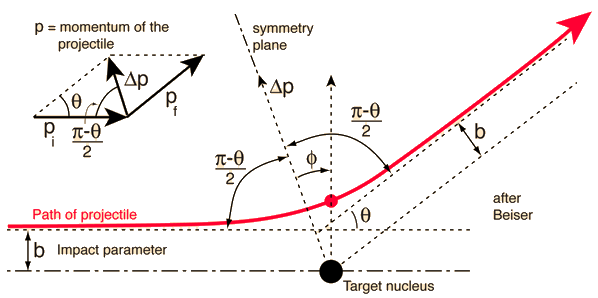
\includegraphics[width=\linewidth]{./lect18/1.png}
\end{center}

$$E = \frac{1}{2}mv_0^2$$

Since angular momentum is conserved, we can measure it far form center of force:
$$l = \left|\vec{r} \times \vec{p}_0 \right| = bmv_0 = b\sqrt{2mE}$$
Denote number of particles arriving to $d\Omega$, a ring acquired by rotating $d\theta$ around the axis, by $dN$. Define flux of particles as $I_0$, number of particles per unit area in unit time in ray. We want to find $\theta(b)$. We can acquire that 
$$\varphi = \int_{r_{min}}^\infty \frac{l dr}{r^2 \sqrt{2m \left(E-V(r)-\frac{l^2}{2mr^2}\right)}}$$
\paragraph{Example}
$V(r) = \frac{\alpha}{r}$. Since $E=mv_0^2$ and $l=mv_0b$:
$$\varphi = \int_{r_{min}}^\infty \frac{l dr}{r^2 \sqrt{2m \left(E-V(r)-\frac{l^2}{2mr^2}\right)}} = \int_{r_{min}}^\infty \frac{b dr}{r^2 \sqrt{1-\frac{b^2}{r^2}-\frac{2\alpha }{mv_0^2 r}}} = \cos^{-1} \left(\frac{\frac{\alpha }{mv_0^2b}}{\sqrt{1+\left(\frac{\alpha }{mv_0^2b}\right)^2}}\right)$$
Denote $x=\frac{\alpha}{mv_0^2b}$:
$$\cos \varphi  =  \frac{x}{\sqrt{1+x^2}}$$
$$\cos^2 \varphi  =  \frac{x^2}{1+x^2}$$
$$\cos^2 \varphi + x^2\cos^2 \varphi  =  x^2$$
$$\cos^2 \varphi = x^2(1-\cos^2\varphi)$$
$$\frac{1}{x^2} = \tan^2 \varphi $$
$$\left(\frac{\alpha}{mv_0^2b}\right)^2 = \frac{1}{\tan^2 \varphi }$$
$$b^2 = \frac{\alpha^2}{m^2v_0^4}\tan^2 \varphi$$
Since angle of incidence is equal to angle of reflection, 
$$b^2 = \frac{\alpha^2}{m^2v_0^4}\cot^2 \frac{\theta}{2}$$
and generally from this equality
$$2\varphi + \theta = 2\pi$$
\subsection{Cross section of scattering}
Lets calculate number of particles going to element of solid angle element $d\Omega=\sin \theta d\theta d\varphi$ (here $\theta$ and $\varphi$ are ones of spherical coordinates) per unit time, i.e. $\frac{dN}{dt}$:
$$\frac{dN}{dt} = \frac{dN}{dt} \frac{d\Omega}{d\Omega} = \frac{dN}{dt} \frac{d\Omega}{d\Omega} \frac{d\sigma}{d\sigma} = \underbrace{\frac{dN}{dt d\sigma}}_{I_0} \cdot \underbrace{\frac{d\sigma}{d\Omega}}_{\parbox{2cm}{\scriptsize \centering differential cross section of scattering}} \cdot d\Omega$$
Thus
$$\frac{d\sigma}{d\Omega} d\Omega = \frac{1}{I_0}\frac{dN}{dt}$$
Now, from geometry:
$$d\sigma = 2\pi b db$$
$$d\Omega = 2\pi \sin \theta d\theta$$
Thus
$$\frac{d\sigma}{d\Omega} = \frac{2\pi b db}{2\pi \sin \theta |d\theta|} = \frac{b(\theta)}{\sin(\theta)} \left|\frac{db}{d\theta}\right|$$
\paragraph{Retherford scattering}
For Retherford scattering

$$b^2 = \frac{\alpha^2}{m^2v_0^4}\cot^2 \frac{\theta}{2}$$
By multiplying by $\frac{1}{2}$ and differentiating both sides
$$\frac{1}{2}\frac{d}{d\theta}b^2 = b\frac{db}{d\theta} = \frac{1}{2} \frac{\alpha^2}{m^2v_0^4}\frac{\cos \frac{\theta}{2}}{\sin^3  \frac{\theta}{2}}$$
$$\frac{d\sigma}{d\Omega} = \frac{2\pi b db}{2\pi \sin \theta |d\theta|} = \frac{ b\frac{db}{d\theta}}{\sin(\theta)} = \frac{1}{2} \frac{\alpha^2}{m^2v_0^4}\frac{1}{\sin\theta} \frac{\cos \frac{\theta}{2}}{\sin^3  \frac{\theta}{2}} = \frac{\alpha^2}{4m^2v_0^4}\frac{1}{\sin^4  \frac{\theta}{2}} $$

By substituting $\alpha = z_1z_2e^2$ and $E= \frac{mv^2}{2}$:
$$\frac{d\sigma}{d\Omega}  =\left( \frac{z_1z_2 e^2}{2E}\right)^2\frac{1}{4\sin^4  \frac{\theta}{2}} $$

\paragraph{Claim}
Total cross section of scattering is
$$\sigma_T = \int \frac{d\sigma}{d\Omega} d\Omega$$

\section{Rigid body}
Rigid body is set of points such that distance between each pair of them is constant - $r_{ij} = c_{ij}$, i.e. a body can't change it's form. 

Denote a position of one of these points in lab frame as $\vec{\mathcal{R}}$, position of point in body frame $\vec{r}$, and position of body in lab frame $\vec{R}$. Lets define infinitesimal transformation of moving and rotation:
$$d\vec{\mathcal{R}} = d\vec{R} + d\vec{\varphi} \times \vec{r}$$ 
Where $d\vec{\varphi}$ is angle of rotation and $d\vec{R} $ displacement of origin.
Then
$$\vec{v} = \frac{d\vec{\mathcal{R}}}{dt} = \frac{d\vec{R}}{dt} + \frac{d\vec{\varphi}}{dt} \times \vec{r}$$
Define $\vec{V} = \frac{d\vec{R}}{dt} $ and $\vec{\Omega} = \frac{d\vec{\varphi}}{dt}$:
$$\vec{v} = \vec{V} + \vec{\Omega} \times \vec{r}$$


\paragraph{$\Omega$ is independent on point of reference}
Suppose we have two reference points, with positions $\vec{r}_1$ and $\vec{r}_2$:
$$\vec{r}_2 = \vec{r}_1 + \vec{a}$$
$$\vec{v} = \vec{V}+ \Omega \times \vec{r}_2 = \vec{V}+ \Omega \times (\vec{r}_1+\vec{a}) = \underbrace{\vec{V}+\Omega \times \vec{a}}_{_{\parbox{2cm}{\scriptsize \centering Velocity of new reference point}}} \Omega \times \vec{r}_1$$

\paragraph{Kinetic energy of rigid body}
\begin{align*}
T = \sum \frac{1}{2}m_i\vec{v}_i^2 = \sum \frac{1}{2}m_i\left(\vec{V} + \vec{\Omega} \times \vec{r}_i\right)^2 = \sum \frac{1}{2}m_i\vec{V}^2 + \sum m_i\vec{V} \left(\vec{\Omega} \times \vec{r}_i\right)+ \sum \frac{1}{2}m_i \left(\vec{\Omega} \times \vec{r}_i\right)^2 =\\= \frac{1}{2}MV^2 + \vec{V} \cdot \left(\vec{\Omega} \times \sum m_i \vec{r}_i\right) + \sum \frac{1}{2}m_i \left(\vec{\Omega} \times \vec{r}_i\right)^2
\end{align*}

If we choose center of mass, i.e. $\sum m_i \vec{r}_i$ and thus:
\begin{align*}
T = = \frac{1}{2}MV^2 + \sum \frac{1}{2}m_i \left(\vec{\Omega} \times \vec{r}_i\right)^2 = T_{cm} + T_{rot}
\end{align*}
$$ \left(\vec{\Omega} \times \vec{r}\right)^2 = \vec{\Omega}^2 \vec{r}^2 - \left(\vec{\Omega} \vec{r}\right)^2 = \Omega_i\Omega_i r^2 - \Omega_i r_i \Omega_j r_j = \Omega_i\Omega_j r^2 \delta_{ij} - \Omega_i r_i \Omega_j r_j $$
(Note $\sum_i x = \sum_j \sum_i x \delta_{ij}$)
In continuous limit:
$$T_{rot} = \frac{1}{2} \rho(\vec{r}) \left(\vec{\Omega} \times \vec{r}\right)^2  d\vec{r} = \frac{1}{2} \int \rho(\vec{r})  \left[\Omega_i\Omega_j r^2 \delta_{ij} - \Omega_i r_i \Omega_j r_j\right] d\vec{r} = \frac{1}{2}\Omega_i \Omega_j \underbrace{\int \rho(\vec{r})( r^2 \delta_{ij} -  r_i r_j )d\vec{r}}_{I_{ij}} $$

$I$ is tensor of inertia
$$I = \begin{pmatrix}
\int \rho(\vec{r}) (y^2+z^2) d\vec{r} & -\int \rho(\vec{r}) xy d\vec{r} & -\int \rho(\vec{r}) xz d\vec{r}\\ 
-\int \rho(\vec{r}) xy d\vec{r} & \int \rho(\vec{r}) (x^2+z^2) d\vec{r} & -\int \rho(\vec{r}) yz d\vec{r}\\
-\int \rho(\vec{r}) xz d\vec{r} & -\int \rho(\vec{r}) yz d\vec{r} & \int \rho(\vec{r}) (x^2+y^2) d\vec{r}  \\
\end{pmatrix}$$

\subsubsection{Examples of inertia tensor calculation}
\paragraph{}
A square with two masses $m$ in opposite vertices (second and forth quarter) and $2m$ in two others, with $z=0$.
$$I_{xx} = \sum_i m_i(y^2_i+z^2_i) = \sum_i m_i y_i^2 = 6ma^2$$
$$I_{yy} = \sum_i m_i(x^2_i+z^2_i) = \sum_i m_i x_i^2 = 6ma^2$$
$$I_{zz} = \sum_i m_i(x^2_i+y^2_i) =  12ma^2$$
Now the mixed terms
$$I_{yx} = I_{xy} = \sum_i -m_ix_iy_i = -2ma^2 -2ma^2 + ma^2 + ma^2 = -2ma^2$$
$$I_{xz} = I_{yz} = I_{zx} = I_{zy} = 0$$
Thus
$$I = \begin{pmatrix}
6ma^2&-2ma^2&0\\
-2ma^2&6ma^2&0\\
0&0&12ma^2
\end{pmatrix}$$
\paragraph{}
Now the same system with axis rotated by $\frac{\pi}{4}$:
$$I_{xx} = \sum_i m_i(y^2_i+z^2_i) = \sum_i m_i y_i^2 = 8ma^2$$
$$I_{yy} = \sum_i m_i(x^2_i+z^2_i) = \sum_i m_i x_i^2 = 4ma^2$$
$$I_{zz} = \sum_i m_i(x^2_i+y^2_i) =  12ma^2$$

Now the mixed terms
$$I_{yx} = I_{xy} = I_{xz} = I_{yz} = I_{zx} = I_{zy} = 0$$
Thus
$$I = \begin{pmatrix}
8ma^2&0&0\\
0&4ma^2&0\\
0&0&12ma^2
\end{pmatrix}$$
\paragraph{Principal axes of inertia}
Since tensor of inertia is symmetrical, it's diagonalizable by orthogonal matrix, thus we can find such axex that $I$ is diagonal in it. We call it principal axes of inertia. 

If a body has a symmetry axis, it has to be on of principal axes.
\paragraph{Continuous case}
A uniform box of size $2a\times 2b \times 2c$ with axes of symmetry. 
\begin{align*}
I_{xx} = \iiint \rho (y^2+z^2) dxdydz = \rho \int_{-a}^{a} dx \int_{-b}^b\int_{-c}^c y^2 + z^2 dz dy = 2\rho a  \int_{-b}^b\int \left[y^2z + \frac{z^3}{3}\right]_{-c}^c   dy =\\= 2\rho a  \int_{-b}^b\int \left[y^2z + \frac{z^3}{3}\right]_{-c}^c   dy = 4\rho a \left(c+\frac{c^3}{3}\right)\int_{-b}^b y^2  dy = 8abc\rho \left(\frac{b^3}{3}+\frac{c^3}{3}\right) = M\left(\frac{b^3}{3}+\frac{c^3}{3}\right)
\end{align*}
Similarly for $I_{yy}$ and $I_{zz}$.

$$I_{xy} = \iint \rho xy dxdydz = 0$$
Can be seen from symmetry, thus

$$I = \begin{pmatrix}
\frac{b^3}{3}+\frac{c^3}{3}&0&0\\
0&\frac{a^3}{3}+\frac{c^3}{3}&0\\
0&0&\frac{a^3}{3}+\frac{b^3}{3}
\end{pmatrix}M$$
\paragraph{Principal axes of inertia}
$$\vec{\Omega} = (\Omega_1, \Omega_2, \Omega_3)$$
Since
$$T  = T_{cm} + \frac{1}{2} \Omega I \Omega = T_{cm} + \frac{1}{2 } \left( I_1\Omega_1^2+ I_2\Omega_2^2+ I_3\Omega_3^2 \right)$$

\paragraph{Translation of axis}
$$\vec{r} = \vec{r}' + \vec{a}$$
Where $r'$ is in center of mass system.
\begin{align*}
I_{ik} = \int \rho \left({r'}^2 \delta_{ik} -r_i'r_k' \right) d\vec{r}' = \int \rho \left({\left(r'-a\right)}^2 \delta_{ik} -(r_i'-a_i)(r_k'-a_k) \right) d\vec{r}' =\\= I_{ik}' + \int \rho \left(\left(-2r'a + a^2\right) \delta_{ik} -(-a_ir_i'-a_kr_k'+a_ia_k) \right) d\vec{r}' =\\= I_{ik}' + \int \rho \left( a^2 \delta_{ik} - a_ia_k \right) d\vec{r}' = I_{ik}' + M \left( a^2 \delta_{ik} - a_ia_k \right) 
\end{align*}

\subsection{Angular momentum of rigid body}
Denote angular momentum around center of mass as $\vec{M}$.
$$\vec{M} = \sum m_i \vec{r}_i \times \vec{v}_i = \int \rho(\vec{r}) \left( \vec{r} \times \vec{v} \right) d\vec{r}$$
From $\vec{v} = \vec{V} + \vec{\Omega} \times \vec{r}$:
$$\vec{M} = \int \rho(\vec{r}) \left( \vec{r} \times \vec{v} \right) dxdydz = \int \rho(\vec{r}) \left( \vec{r} \times \left(\vec{V} + \vec{\Omega} \times \vec{r}\right) \right) dxdydz  = \int \rho(\vec{r}) \left( \vec{r} \times \vec{V} + \vec{r} \times \vec{\Omega} \times \vec{r}\right) dxdydz $$
From $\vec{a} \times (\vec{b} \times \vec{c}) = \vec{b}(ac) - \vec{c}(ab)$:
\begin{align*}
\vec{M} = \underbrace{\int \rho(\vec{r})  \vec{r} \times \vec{V} dxdydz}_{0} +\int \rho(\vec{r})\left(\vec{\Omega} r^2 + \vec{r} \left(\vec{\Omega} \cdot \vec{r}\right)\right) dxdydz =\\= \int \rho(\vec{r})\left(\vec{\Omega} r^2 + \vec{r} \left(\vec{\Omega} \cdot \vec{r}\right)\right) dxdydz =  \int \rho(\vec{r})\left(\vec{\Omega} r^2 + \vec{r} \left(\vec{\Omega} \cdot \vec{r}\right)\right) dxdydz
\end{align*}
$$M_i =\int \rho(\vec{r})\left(\vec{\Omega}_i r^2 + \vec{r}_j \left(\vec{\Omega}_i \cdot \vec{r}_i\right)\right) dxdydz = \int \rho(\vec{r})\left(\vec{\Omega}_j \delta_{ij} r^2 + \vec{r}_i \left(\vec{\Omega}_j \cdot \vec{r}_j\right)\right) dxdydz = I_{ij} \Omega_j $$
That means
$$\vec{M} = I\vec{\Omega}$$
\paragraph{Note} $$\vec{M} \not\parallel \vec{\Omega}$$
\paragraph{Symmetrical }
Lagrangian is
$$\mathcal{L}  = \frac{1}{2} MV^2 + \frac{1}{2} I_{ik} \Omega_i \Omega_k$$
$$\dot{\vec{M}} = \frac{d}{dt} \left( \sum m_i \vec{r}_i \times v_i \right) = \sum m_i \vec{v}_i \times \vec{v}_i + \sum \vec{r}_i \times m\dot{\vec{v}}_i = \sum \vec{r}_i \times \dot{\vec{p}}_i = \sum \vec{r}_i \times \vec{f}_i = \vec{N} $$

\paragraph{}
Suppose $\hat{z}$ is axis of symmetry, then we can choose $\hat{x}$ and $\hat{y}$ such that $M_y=0$ and thus $\Omega_y = 0$. For point $\vec{r} = (0,0,r)$:
$$\vec{v} = \vec{V} + \vec{\Omega} \times \vec{r} = \vec{\Omega} \times \vec{r}  = (0, -\Omega_1 r, 0)$$
\subsection{Euler angles}
\begin{center}
	\includesvg[eps,svgpath = lect22/,width=0.5\linewidth]{Eulerangles}
\end{center}
We do three rotations - around $z$ axis by $\varphi$, then around $x$ axis by $\theta$, and once again around $z$ axis by $\psi$.
Denote
$$D = \begin{pmatrix}
\cos \varphi&\sin \varphi & 0\\
-\sin \varphi & \cos \varphi & 0\\
0&0&1
\end{pmatrix}$$
$$C = \begin{pmatrix}
1&0&0\\
0&\cos \theta&\sin \theta \\
0&-\sin \theta & \cos \theta \\
\end{pmatrix}$$
$$B = \begin{pmatrix}
\cos \psi&\sin \psi & 0\\
-\sin \psi & \cos \psi & 0\\
0&0&1
\end{pmatrix}$$
Now
$A= BCD$
and
$$\begin{pmatrix}
x'\\y'\\z'
\end{pmatrix} = A\begin{pmatrix}
x\\y\\z
\end{pmatrix}$$

\paragraph{Calculation of angular velocity}
$$0\leq \theta < \pi$$
$$0\leq \varphi, \psi < 2\pi$$
In body's system
$$\vec{\dot{\psi}} = \begin{pmatrix}
0\\0\\\dot{\psi}
\end{pmatrix}$$
$$\vec{\dot{\theta}} = \begin{pmatrix}
\dot{\theta}\cos \psi\\\dot{\theta}\sin \psi\\0
\end{pmatrix}$$
$$\vec{\dot{\varphi}} = \begin{pmatrix}
\dot{\varphi}\sin \theta \sin \varphi\\\dot{\varphi}\sin \theta \cos \varphi\\\dot{\varphi} \cos \theta
\end{pmatrix}$$
Thus
$$\vec{\Omega} = \begin{pmatrix}
\dot{\varphi}\sin \theta \sin \varphi+\dot{\theta}\cos \psi\\\dot{\varphi}\sin \theta \cos \varphi-\dot{\theta}\sin \psi\\\dot{\varphi} \cos \theta+\dot{\psi}
\end{pmatrix}$$

Find kinetic energy
$$T_{rot} = \frac{1}{2} I_1 \left( \dot{\varphi}\sin \theta \sin \varphi+\dot{\theta}\cos \psi \right)^2 + \frac{1}{2} I_2 \left( \dot{\varphi}\sin \theta \cos \varphi-\dot{\theta}\sin \psi \right)^2 
+ \frac{1}{2} I_3 \left( \dot{\varphi} \cos \theta+\dot{\psi} \right)^2 $$
For symmetrical gyroscope ($I_1=I_2$)
$$T_{rot} = \frac{1}{2} I_1 \left( \dot{\varphi}^2 \sin^2 \theta + \dot{\theta}^2  \right) +  \frac{1}{2} I_3 \left( \dot{\varphi} \cos \theta + \dot{\psi}  \right)^2$$
\paragraph{Lagrangian}
We have 6 degrees of freedom: $\vec{R}$, $\theta$, $\varphi$, $\psi$.
$$L = \frac{1}{2} M \vec{\dot{R}}^2 + \frac{1}{2} I_i \Omega_i^2 + U\left( \vec{R}, \theta, \varphi, \psi \right)$$
For $\vec{R}$:
$$\vec{\dot{P}}=M\vec{\ddot{R}} = -\vec{\nabla}_R U = \vec{F}$$
\paragraph{Movement equations from momentum and angular momentum}
$$\vec{\dot{P}} = \sum_i m_i \vec{v}_i = \sum_i \vec{f}_i = \vec{F}$$
For angular momentum:
$$\vec{\dot{M}} = \sum_i m_i \underbrace{\vec{\dot{r}}_i \times \vec{v}_i}_{0} + m_i \vec{r}_i \times \vec{\dot{v}}_i =  \sum_i m_i \vec{r}_i \times \vec{\dot{v}}_i =  \sum_i \vec{r}_i \times \vec{\dot{p}}_i = \vec{N}$$
$$\frac{d}{dt} \vec{M} = \vec{N}$$
$$\left[\frac{d}{dt} \vec{M}\right]_{\text{lab}} = \left[\frac{d}{dt} \vec{M}\right]_{\text{body}} + \vec{\Omega} \times \vec{M}$$
If we take inertial system such that a given moment axes are same as axes of body, after rotation, if $\vec{M}$ in body's FOR is unchanged, and thus is equal $\vec{\Omega}\times \vec{M}$.
$$\frac{d\vec{M}}{dt}_i = \dot{M}_i + \epsilon_{ijk} \Omega_j M_k = I_i \dot{\Omega}_i + \epsilon_{ijk} \Omega_j I_k \Omega_k = N_i$$
Then Euler equations are;
$$\begin{cases}
 I_1 \dot{\Omega}_1 + \Omega_2 \Omega_3 (I_3-I_2) = N_1\\
 I_2 \dot{\Omega}_2 + \Omega_1 \Omega_3 (I_1-I_3) = N_2\\
 I_3 \dot{\Omega}_3 + \Omega_1 \Omega_2 (I_2-I_1) = N_3\\
\end{cases}$$

\paragraph{Example}
Symmetric gyroscope: in body's system $\vec{N} = 0$, then
$$\begin{cases}
I_1 \dot{\Omega}_1 + \Omega_2 \Omega_3 (I_3-I_1) = 0\\
I_1 \dot{\Omega}_2 + \Omega_1 \Omega_3 (I_1-I_3) = 0\\
I_3 \dot{\Omega}_3  = 0\\
\end{cases}$$
We can easily see that
$\Omega_3 = \frac{M_3}{I_3}$. Define
$$\omega = \Omega_3 \frac{I_1+I_3}{I_1}$$
Then
$$\begin{cases}
\dot{\Omega}_1 = -\omega \Omega_2\\
\dot{\Omega}_2 = -\omega \Omega_1\\
\end{cases}$$
Differentiating:
$$\begin{cases}
\ddot{\Omega}_1 = -\omega^2 \Omega_2\\
\ddot{\Omega}_2 = -\omega^2 \Omega_1\\
\end{cases}$$
Then
$$\begin{cases}
\Omega_1  =  A \cos \left( \omega t+ \Psi_0  \right)\\
\Omega_2  =   A \sin \left( \omega t+ \Psi_0  \right)\\
\Omega_3  =  \frac{M_3}{I_3}\\
\end{cases}$$

The symmetry axis is making circular motion around vertical axis. Lets find precession frequency:
$$\omega_{pr} = \frac{V}{R} = \frac{\Omega_1R_3}{R_3 \sin \theta}  = \frac{\Omega_1}{\sin \theta}  = \frac{\Omega_1I_1}{I_1\sin \theta} = \frac{M_1}{I_1\sin \theta} = \frac{M\sin \theta}{I_1\sin \theta} = \frac{M}{I_1}$$
\paragraph{Assymetric gyroscope}
$\vec{N}= 0$ and $I_1 < I_2 < I_3$. From conservations:
$$E = \frac{1}{2} \left( I_1\Omega_1^2 + I_2 \Omega_2^2 + I_3\Omega_3^2 \right) = \text{const}$$
$$m^2 = M_1^2+M_2^2+M_3^2 = \text{const}$$
Then
$$\frac{M_1^2}{2EI_1}+\frac{M_2^2}{2EI_2}+\frac{M_3^2}{2EI_3} = 1$$

The body trajectory moves on intersection of ellipsoid and sphere:
\begin{center}
	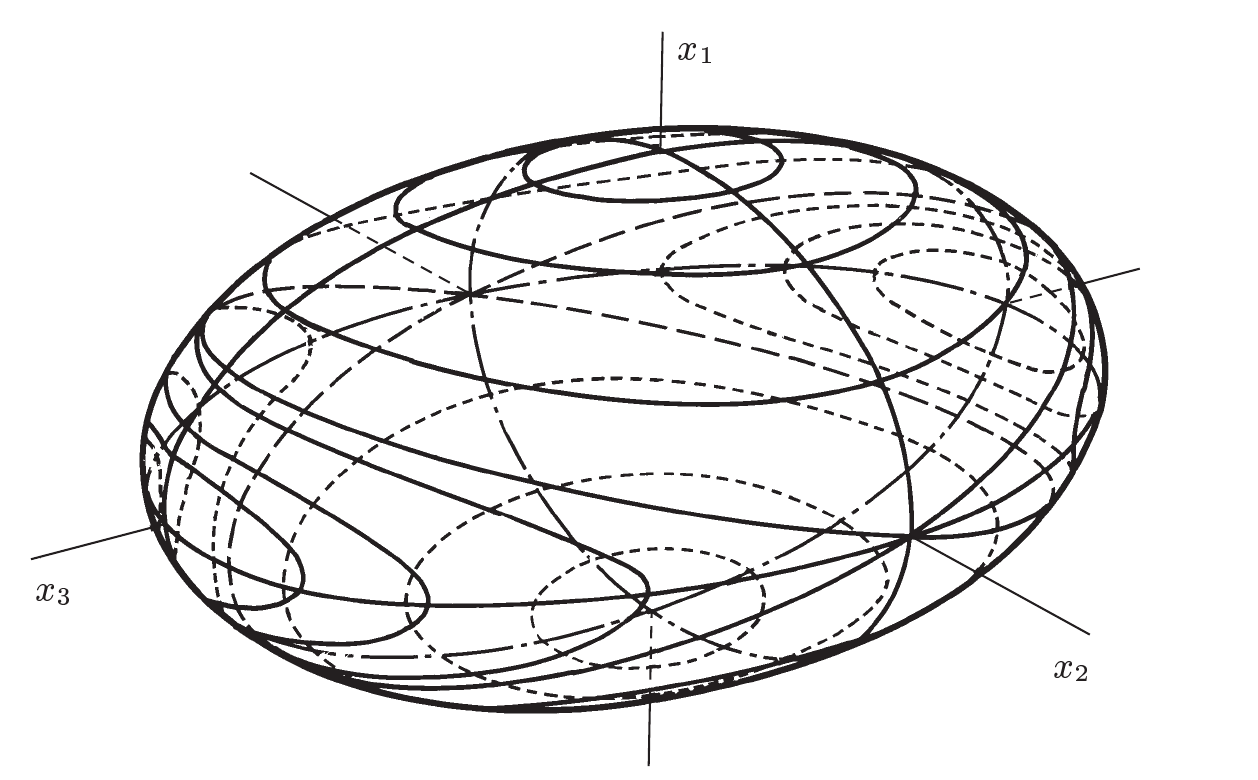
\includegraphics[width=\linewidth]{./lect23/1.png}
\end{center}
Those are intersections of ellipsoid and spheres of different radii.

If we denote 
$$\begin{cases}
\alpha_1 = -\frac{I_3-I_2}{I_1} < 0\\
\alpha_2 = -\frac{I_1-I_3}{I_2} > 0\\
\alpha_3 = -\frac{I_2-I_1}{I_3} < 0
\end{cases}$$
Suppose rotation close to one of the axis:
$$\begin{cases}
\Omega_1 = \omega_1\\
\Omega_2 = \Delta\omega_2\\
\Omega_3 =  \Delta\omega_3\\
\end{cases} \quad \Delta \omega_2, \Delta \omega_3 \ll \omega$$
Then Euler equations are:
$$\begin{cases}
\dot{\omega} = \Omega_1\Omega_2\alpha_3 = 0\\
\Delta \dot{\omega}_1 =\omega \Delta \omega_2 \alpha_1\\
\Delta \dot{\omega}_2  =\omega \Delta \omega_1 \alpha_2\\
\end{cases}$$
Thus
$$\Delta \ddot{\omega}_1 = \omega^2 \alpha_1 \alpha_2 \Delta \omega_1 \omega = \text{const}$$
and depending on positive or negative coefficient 

\subsection{Symmetric gyroscope with gravitation}
\begin{center}
	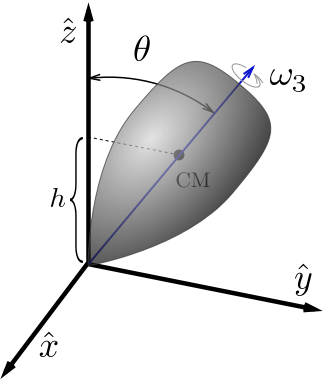
\includegraphics[width=0.3\linewidth]{./lect24/1.png}
\end{center}
Lets move from center of mass to fixed point, then
$$I^* = \begin{pmatrix}
I_1&0&0\\0&I_2&0\\0&0&I_3
\end{pmatrix}+\begin{pmatrix}
\mu a^2&0&0\\0&\mu a^2&0\\0&0&0
\end{pmatrix}$$
$$\mathcal{L} = T -V$$
$$T = T_{rot} = \frac{1}{2}I^{*}_i \Omega_i^2$$
$$V = \mu gh = \mu ga\cos \theta$$
$$\mathcal{L} = \frac{1}{2} I^*_1 \left(\dot{\theta}^2 + \dot{\varphi}^2 \sin^2 \theta\right) + \frac{1}{2} I^*_3 \left( \dot{\varphi} \cos \theta + \dot{\psi}\right)^2 - \mu g a \cos \theta$$
We can calculate momenta:
$$\begin{cases}
P_\theta = I^*_1 \dot{\theta}\\
P_\psi = I^*_2 \left(\psi\right) = L_3\\
P_\varphi = I^*_1 \dot{\varphi} sin^2 \theta + I^*_3 \left(\dot{\varphi}  \cos \theta + \dot{\psi}\right)\cos \theta = L_z
\end{cases}$$
The conserved values are canonical momenta of $\psi$ (angular momentum around $3$-axis) and $\varphi$  (angular momentum around $z$-axis)  and energy. 

$$H  = \frac{P_\theta^2}{2I^*_1} + \frac{\left(P_\varphi - P_\psi\cos \theta\right)^2}{2I^*_1 \sin^2 \theta} + \frac{P_\psi^2}{2I^*_3} +\mu ga\cos \theta$$
Define
$$U_{eff} (\theta) = \frac{\left(L_z - L_3 \cos \theta \right)^2}{2I^*_1 \sin^2 \theta} - \mu g a (1-\cos \theta ) + \left( \frac{L_3^2}{2I^*_3}  +\mu ga  \right)$$
Then
$$H(\theta, P_\theta) = \frac{P_\theta^2}{2I^*_1} + U_{eff} = E$$
$$\frac{d\theta}{dt} = \frac{\partial H}{\partial P_\theta} = \frac{P_\theta}{I^*_1} = \frac{\sqrt{2I^*_1\left(E-U_{eff}(\theta)\right)}}{I^*_1}$$
$$t  =\int \frac{I^*_1d\theta}{\sqrt{2I^*_1\left(E-U_{eff}(\theta)\right)}}$$
That allows us to find $\theta$. For $\varphi$ and $\psi$:
$$\begin{cases}
\dot{\varphi} = \frac{L_z-L_3\cos \theta}{I^*_1 \sin^2 \theta}\\
\dot{\psi} = \frac{L_3}{I^*_3}-\dot{\varphi}\cos \theta
\end{cases}$$

\begin{center}
	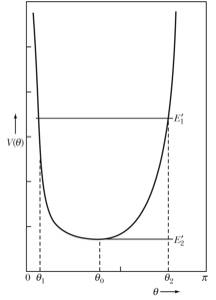
\includegraphics[width=0.3\linewidth]{./lect24/3.jpg}
\end{center}
Since effective potential goes to infinity in $\theta=0$ and $\theta=\pi$ (given $L_z\neq L_3$), the equation $E=U_{eff}$ has two solutions $\theta_1$ and $\theta_2$ and gyroscope will oscillate between them. 

If $L_z-L_3\cos \theta > 0$ for all $\theta$, $\dot{\varphi} $ doesn't change it sign and we get nutation. If its value changes sign for some $\theta$, then we get second case, in which the trajectory has loops. In the limit, if $\dot{\varphi} = 0$ exactly for $\theta_2$ (or $\theta_1$) we get third type of trajectories.

\begin{center}
	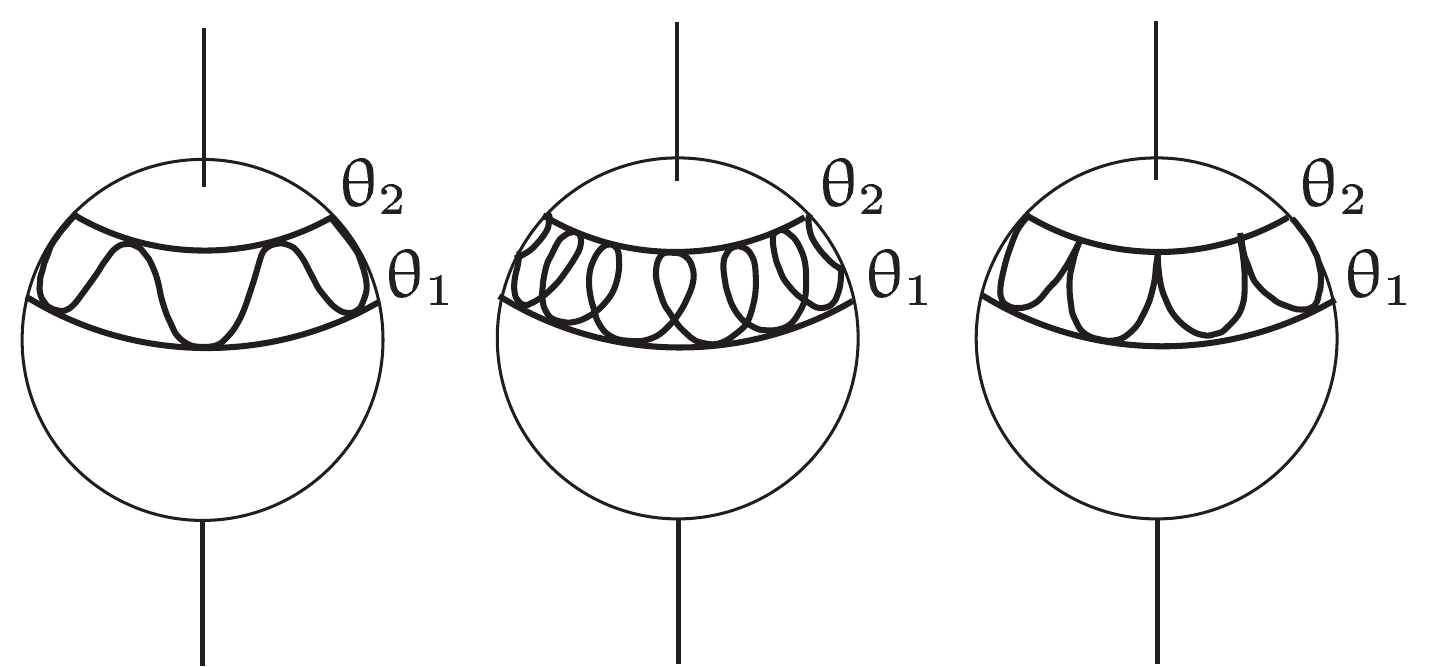
\includegraphics[width=\linewidth]{./lect24/2.png}
\end{center}

\section{Non-integrable systems}
\subsection{Harmonic oscillator. Angle-Action variable}
Hamiltonian of harmonic oscillator is:
$$H = \frac{p^2}{2m} + \frac{1}{2} m\omega^2 q^2$$
$$\begin{cases}
\dot{p} = -\frac{\partial H}{\partial q} = -m\omega^2 q \\
\dot{q} = \frac{\partial H}{\partial p} = \frac{p}{m}
\end{cases}$$
Thus
$$\begin{cases}
q = A\cos \left(\omega t  -\theta_0\right)\\
p = m\omega A\sin \left(\omega t  -\theta_0\right)
\end{cases}$$

The movement in phase space is ellipses.

Now define new coordinates, $I$ -- action variable and $\theta$ -- angle variable, in the following way:
$$\begin{cases}
q = \sqrt{\frac{2I}{m\omega}}\sin \theta\\
p = \sqrt{2Im\omega}\cos \theta
\end{cases}$$
We can check that transformation is canonical by Poisson brackets:
$$\left\{ q,p \right\}_{\theta, I} = \left\{ \sqrt{\frac{2I}{m\omega}}\sin \theta,\sqrt{2Im\omega}\cos \theta \right\}_{\theta, I} = 2\left\{ \sqrt{I}\sin \theta,\sqrt{I}\cos \theta \right\}_{\theta, I}  = 2 \cdot \left[ \sqrt{I} \cos \theta \cdot \frac{\cos \theta}{2\sqrt{I}}  + \frac{\sin \theta}{2\sqrt{I}} \cdot \sqrt{I} \sin \theta\right] = 1$$

Now the Hamiltonian is 
$$H = \omega I$$
And Hamilton equations are
$$\begin{cases}
\dot{I} = 0\\
\dot{\theta} = \omega
\end{cases} \Rightarrow \begin{cases}
I = \text{const}\\
\theta = \omega t + \theta_0
\end{cases}
$$

\paragraph{Definition}
System with $n$ degrees of freedom is called integrable if exists canonical transformation 
$(q_i,p_i) \to (\theta_i, I_i)$ such that $H = H(I_i, \dots, I_n)$. In this case 
$$\begin{cases}
\dot{I}_i = 0\\
\dot{\theta}_i = \omega_i(I)
\end{cases} \Rightarrow \begin{cases}
I_i = \text{const}\\
\theta_i = \omega_i(I) t + \theta_{0i}
\end{cases}
$$
\subsection{Angle-Action variable for systems with one degree of freedom}
$$H = \frac{p^2}{2m} + V(q)$$
$H$ is energy and constant, also suppose $q$ is bounded: $q_1 \leq q \leq q_2$.

So we are searching for canonical transformation such that $H = H(I)$. Define
$$I = \frac{1}{2\pi} \oint p dq$$
$$p = \sqrt{2m(E-V(q))}$$
$$dt = \frac{dq}{\dot{q}} = \sqrt{\frac{m}{2}}\frac{dq}{\sqrt{E-V(q)}}$$
Now, $T=\frac{2\pi}{\omega}$:
$$\frac{2\pi}{\omega} = \oint \sqrt{\frac{m}{2}}\frac{dq}{\sqrt{E-V(q)}} = 2\sqrt{\frac{m}{2}} \oint  \frac{d}{dE}\sqrt{E-V(q)} dq = =\frac{d}{dE} \left(\oint  \sqrt{2m(E-V(q))} dq\right) = \frac{d}{dE}\oint p dq = 2\pi \frac{d}{dE}  I $$
Thus
$$\frac{dE}{dI} = \omega $$
\subsection{2D movement}
\subsubsection{Integrable system}
Suppose system is integrable and movement is bounded. Then
$$\begin{cases}
I_1 = \text{const}\\I_2 = \text{const}\\\theta_1 = \omega_1(I) t + \theta_{01}\\\theta_1 = \omega_2(I) t + \theta_{02}
\end{cases}$$

Now, both $\theta$ are periodical, we can say that they move on torus.
\end{document}
